\documentclass[oneside]{book}
\usepackage[utf8]{inputenc}
\usepackage[T1]{fontenc}
\usepackage[brazil,english]{babel}
\usepackage[a4paper, total={6in, 8in}]{geometry}
\usepackage{listings}
\usepackage{xcolor}
\usepackage{multicol}
\usepackage{color}
\usepackage{amsmath}
\usepackage{comment}
\setlength{\columnseprule}{1pt}
\def\columnseprulecolor{\color{black}}
\lstset { %
    language=C++,
    breaklines=true,
    %backgroundcolor=\color{black!5}, % set backgroundcolor
    basicstyle=\footnotesize,% basic font setting
    tabsize=3, % tab space width
}
\geometry{
 a4paper,
 left=10mm,
 right=10mm,
 top=1in,
 bottom=1in,
}
\usepackage{graphicx}

\author{Gabriel Duarte}
\title{Notebook 100^o\\UNIFESO}


\begin{document}
\begin{otherlanguage}{brazil}

\maketitle
\tableofcontents

\chapter{Introdução}

\section{Template}

Digitar o template no inicio da prova. \\
\textbf{NÃO} esquecer de remover o $freopen()$
\begin{multicols}{2}
\begin{lstlisting}
#include <bits/stdc++.h>
using namespace std;
#define all(v) (v).begin(), (v).end()
#define pb push_back
#define fst first
#define snd second
#define debug(x) cout << #x << " = " << x << endl;
typedef long long ll;
typedef pair<int, int> ii;

int main(){
	freopen("in", "rt", stdin);

	return 0;
}
\end{lstlisting}
\end{multicols}

\section{Fast Input}

Em casos extremos mete isso sem medo. 
\begin{multicols}{2}
\begin{lstlisting}
template<class num>inline void rd(num &x)
{
	char c;
	while(isspace(c = getchar()));
	bool neg = false;
	if(!isdigit(c))
		neg=(c=='-'), x=0;
	else
		x=c-'0';
	while(isdigit(c=getchar()))
		x=(x<<3)+(x<<1)+c-'0';
	if(neg)
		x=-x;
}
\end{lstlisting}
\end{multicols}

\section{Bugs do Milênio}

Cortesia da ITA. \\

\begin{multicols}{2}

\textbf{Erros teóricos:}
\begin{itemize}
\itemsep0em
\item Não ler o enunciado do problema com calma.
\item Assumir algum fato sobre a solução na pressa.
\item Não reler os limites do problema antes de submeter.
\item Quando adaptar um algoritmo, atentar para todos os detalhes da estrutura do algoritmo, se devem (ou não) ser modificados (ex:marcação de vértices/estados).
\item O problema pode ser NP, disfarçado ou mesmo sem limites especificados. Nesse caso a solução é bronca mesmo. Não é hora de tentar ganhar o prêmio nobel.
\end{itemize}

\textbf{Erros com valor máximo de variável:}
\begin{itemize}
\itemsep0em
\item Verificar com calma (fazer as contas direito) para ver se o infinito é tão infinito quanto parece. 
\item Verificar se operações com infinito estouram 31 bits.
\item Usar multiplicação de $int$'s e estourar 32 bits (por exemplo, checar sinais usando $a*b > 0$).
\end{itemize}

\textbf{Erros de casos extremos:}
\begin{itemize}
\itemsep0em
\item Testou caso $n=0$? $n=1$? $n=MAXN$? Muitas vezes tem que tratar separado.
\item Pense em todos os casos que podem ser considerados casos extremos ou casos isolados.
\item Casos extremos podem atrapalhar não só no algoritmo, mas em coisas como construir alguma estrutura (ex: lista de adj em grafos).
\item Não esquecer de self-loops ou multiarestas em grafos.
\item Em problemas de caminho Euleriano, verificar se o grafo é conexo.
\end{itemize}

\textbf{Erros de desatenção em implementação:}
\begin{itemize}
\itemsep0em
\item Errar ctrl-C/ctrl-V em código. Muito comum.
\item Colocar igualdade dentro de $if$? ($if(a = 0) continue;$)
\item Esquecer de inicializar variável.
\item Trocar $break$ por $continue$ (ou vice-versa).
\item Declarar variável global e variável local com mesmo nome (é pedir pra dar merda...).
\end{itemize}

\textbf{Erros de implementação:}
\begin{itemize}
\itemsep0em
\item Definir variável com tipo errado ($int$ por $double$, $int$ por $char$).
\item Não usar variável com nome $max$ e $min$.
\item Não esquecer que $.size()$ é unsigned.
\item Lembrar que 1 é $int$, ou seja, se fizer $long \; long \; a \; = \; 1 \; << \; 40;$, não irá funcionar (o ideal é fazer $long \; long \; a \; = \; 1LL \; << \; 40;$).
\end{itemize}

\textbf{Erros em limites:}
\begin{itemize}
\itemsep0em
\item Qual o ordem do tempo e memória? $10^8$ é uma referência para tempo. Sempre verificar rapidamente a memória, apesar de que o limite costuma ser bem grande.
\item A constante pode ser muito diminuída com um algoritmo melhor (ex: húngaro no lugar de fluxo) ou com operações mais rápidas (ex: divisões são lentas, bitwise é rápido)?
\item O exercício é um caso particular que pode (e está precisando) ser otimizado e não usar direto a biblioteca? 
\end{itemize}


\textbf{Erros em doubles:}
\begin{itemize}
\itemsep0em
\item Primeiro, evitar (a não ser que seja necessário ou mais simples a solução) usar $float/double$. E.g. conta que só precisa de 2 casas decimais pode ser feita com inteiro e depois $\% 100$.
\item Sempre usar $double$, não $float$ (a não ser que o enunciado peça explicitamente).
\item Testar igualdade com tolerância (absoluta, e talvez relativa).
\item Cuidado com erros de imprecisão, em particular evitar ao máximo subtrair dois números praticamente iguais.
\end{itemize}

\textbf{Outros erros:}
\begin{itemize}
\itemsep0em
\item Evitar (a não ser que seja necessário) alocação dinâmica de memória.
\item Não usar STL desnecessariamente (ex: vector quando um array normal dá na mesma), mas usar se facilitar (ex: nomes associados a vértices de um grafo - $map<string,int>$) ou se precisar (ex: um algoritmo $O(nlogn)$ que usa $<set>$ é necessário para passar no tempo).
\item Não inicializar variável a cada teste (zerou vetores? zerou variável que soma algo? zerou com zero? era pra zerar com zero, com -1 ou com INF?).
\item Saída está formatada corretamente?
\item Declarou vetor com tamanho suficiente?
\item Cuidado ao tirar o módulo de número negativo. Ex.: $x\%n$ não dá o resultado esperado se x é negativo, fazer $(x\%n + n)\%n$.
\end{itemize}

\end{multicols}

\section{Recomendações gerais}

Cortesia da PUC-RJ. \\

\textbf{ANTES DA PROVA}
\begin{itemize}
\itemsep0em
\item Revisar os algoritmos disponíveis na biblioteca.
\item Revisar a referência STL.
\item Reler este roteiro.
\item Ouvir o discurso motivacional do técnico.
\end{itemize}

\textbf{ANTES DE IMPLEMENTAR UM PROBLEMA}
\begin{itemize}
\itemsep0em
\item Quem for implementar deve relê-lo antes.
\item Peça todas as clarifications que forem necessárias.
\item Marque as restrições e faça contas com os limites da entrada.
\item Teste o algoritmo no papel e convença outra pessoa de que ele funciona.
\item Planeje a resolução para os problemas grandes: a equipe se junta para definir as estruturas de dados, mas cada pessoa escreve uma função.
\end{itemize}

\textbf{DEBUGAR UM PROGRAMA}
\begin{itemize}
\itemsep0em
\item Ao encontrar um bug, escreva um caso de teste que o dispare.
\item Reimplementar trechos de programas entendidos errados.
\item Em caso de RE, procure todos os [, / e \%.
\end{itemize}

\section{Os 1010 mandamentos}

Também cortesia da PUC-RJ.
\\\\
0. Não dividirás por zero.\\
1. Não alocarás dinamicamente.\\
2. Compararás números de ponto flutuante usando EPS.\\
3. Verificarás se o grafo pode ser desconexo.\\
4. Verificarás se as arestas do grafo podem ter peso negativo.\\
5. Verificarás se pode haver mais de uma aresta ligando dois vértices.\\
6. Conferirás todos os índices de uma programação dinâmica.\\
7. Reduzirás o branching factor da DFS.\\
8. Farás todos os cortes possíveis em uma DFS.\\
9. Tomarás cuidado com pontos coincidentes e com pontos colineares.\\

\newpage

\section{Limites da representação de dados}

\begin{table}[h!]
\centering{
\begin{tabular}{|c|c|ccc|c|}
\hline
tipo & bits & mínimo &..& máximo & precisão decimal\\
\hline

char & $8 $	& $0$ &..& $127 $ & $2 $\\
signed char & $8 $& $-128$ &..& $127 	$ & $2 $\\
unsigned char & $8 $ & $0$ &..& $255 $ & $2 $\\
short & $16$ & $-32.768$ &..& $32.767 $ & $4 $\\
unsigned short & $16$ & $0$ &..& $65.535 $ & $4 $\\
int & $32$ 	& $-2 \times 10^9$ &..& $2 \times 10^9 $ & $9 $\\
unsigned int & $32$ & $0$ &..& $4 \times 10^9 $ & $9 $\\
long long & $64$ & $-9 \times 10^{18}$ &..& $9 \times 10^{18} $ & $18$ \\
unsigned long long & $64$ 	& $0$ &..& $18 \times 10^{18} 				$ & $19$ \\

\hline

\end{tabular}
}
\end{table}

\begin{table}[h!]
\centering{
\begin{tabular}{|c|c|c|c|}
\hline
tipo & bits & expoente & precisão decimal \\
\hline
float & 32 & 38 & 6 \\
double & 64 & 308 & 15 \\
long double & 80 & 19.728 & 18 \\

\hline

\end{tabular}
}
\end{table}

\section{Quantidade de números primos de $1$ até $10^n$}

É sempre verdade que $n / ln(n) < pi(n) < 1.26 * n / ln(n)$.

\begin{table}[h!]
\centering{
\begin{tabular}{|c|c|c|}
\hline
$pi(10^1) = 4$ &
$pi(10^2) = 25$ &
$pi(10^3) = 168$ \\
$pi(10^4) = 1.229$ &
$pi(10^5) = 9.592$ &
$pi(10^6) = 78.498$ \\
$pi(10^7) = 664.579$ &
$pi(10^8) = 5.761.455$ &
$pi(10^9) = 50.847.534$ \\

\hline

\end{tabular}
}
\end{table}

\section{Triângulo de Pascal}

\begin{table}[h!]
\centering{
\begin{tabular}{|c|ccccccccccc|}
\hline
$n \backslash p$ & $0$ & $1$ & $2$ & $3$ & $4$ & $5$ & $6$ & $7$ & $8$ & $9$ & $10$ \\
\hline
$0 $ & $1$ &&&&&&&&&&\\
$1 $ & $1$ & $1 $ &&&&&&&&&\\
$2 $ & $1$ & $2 $ & $1 $ &&&&&&&&\\
$3 $ & $1$ & $3 $ & $3 $ & $1$   &&&&&&&\\
$4 $ & $1$ & $4 $ & $6 $ & $4$   & $1$  &&&&&&\\
$5 $ & $1$ & $5 $ & $10$ & $10$  & $5$  & $1$   &&&&&\\
$6 $ & $1$ & $6 $ & $15$ & $20$  & $15$ & $6$   & $1$   &&&&\\
$7 $ & $1$ & $7 $ & $21$ & $35$  & $35$ & $21$  & $7$   & $1$   &&&\\
$8 $ & $1$ & $8 $ & $28$ & $56$  & $70$ & $56$  & $28$  & $8$   & $1$  &&\\
$9 $ & $1$ & $9 $ & $36$ & $84$  & $126$& $126$ & $84$  & $36$  & $9$  & $1$  &\\
$10$ & $1$ & $10$ & $45$ & $120$ & $210$& $252$ & $210$ & $120$ & $45$ & $10$ & $1$\\

\hline

\end{tabular}
}
\end{table}

\begin{table}[h!]
\centering{
\begin{tabular}{|c|c|c|}
\hline
$C(33, 16)$ & $1.166.803.110$ & limite do int \\
$C(34, 17)$ & $2.333.606.220$ & limite do unsigned int \\
$C(66, 33)$ & $7.219.428.434.016.265.740$ & limite do long long \\
$C(67, 33)$ & $14.226.520.737.620.288.370$ & limite do unsigned long long \\
\hline
\end{tabular}
}
\end{table}

\newpage

\section{Fatoriais}

Fatoriais até 20 com os limites de tipo.

\begin{table}[h!]
\centering{
\begin{tabular}{|c|c|c|}
\hline
$0! $ & $1$ & \\
$1! $ & $1$ & \\
$2! $ & $2$ & \\
$3! $ & $6$ & \\
$4! $ & $24$ & \\
$5! $ & $120$ & \\
$6! $ & $720$ & \\
$7! $ & $5.040$ & \\
$8! $ & $40.320$ & \\
$9! $ & $362.880$ & \\
$10!$ & $3.628.800$ & \\
$11!$ & $39.916.800$ & \\
$12!$ & $479.001.600$ & limite do unsigned int \\
$13!$ & $6.227.020.800$ & \\
$14!$ & $87.178.291.200$ & \\
$15!$ & $1.307.674.368.000$ & \\
$16!$ & $20.922.789.888.000$ & \\
$17!$ & $355.687.428.096.000$ & \\
$18!$ & $6.402.373.705.728.000$ & \\
$19!$ & $121.645.100.408.832.000$ & \\
$20!$ & $2.432.902.008.176.640.000$ & limite do unsigned long long \\
\hline

\end{tabular}
}
\end{table}

\section{Tabela ASCII}

\begin{figure}[h]
	\centering
	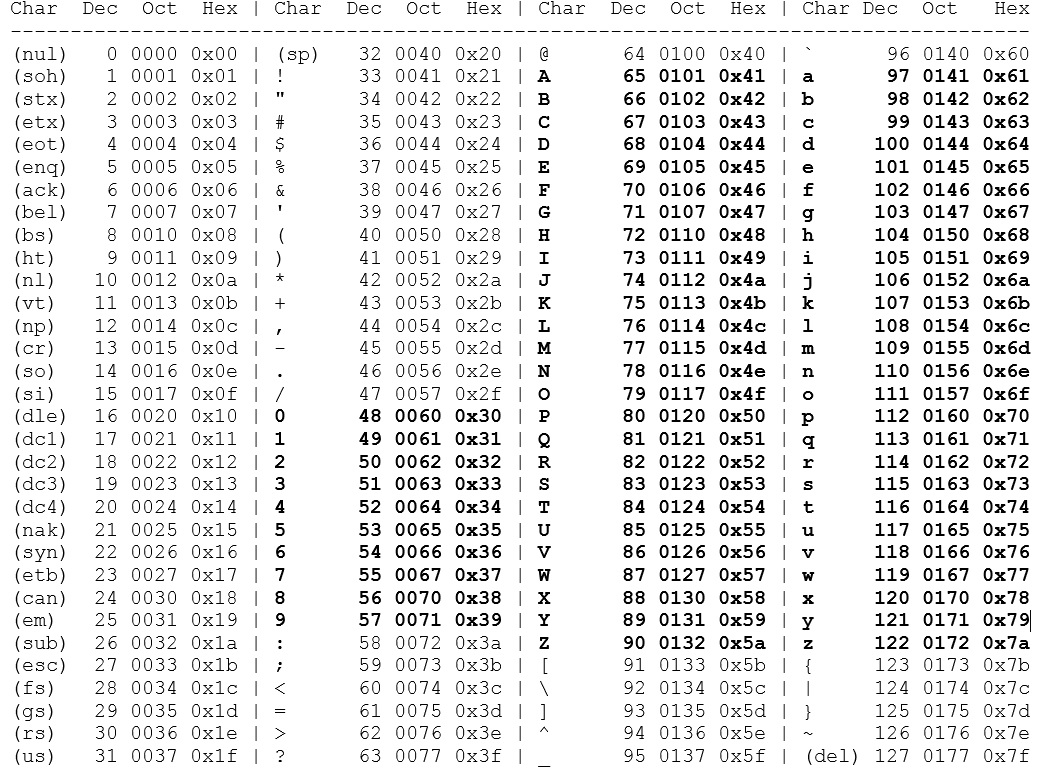
\includegraphics[width=0.68125\textwidth]{ascii.jpg}
\end{figure}

\newpage

\section{Primos até 10.000}

Existem 1.229 números primos até 10.000.

\begin{table}[h!]
\centering{
\begin{tabular}{|c|c|c|c|c|c|c|c|c|c|c|}
\hline
$2   $ & $3   $ & $5   $ & $7   $ & $11  $ & $13  $ & $17  $ & $19  $ & $23  $ & $29  $ & $31  $ \\
$37  $ & $41  $ & $43  $ & $47  $ & $53  $ & $59  $ & $61  $ & $67  $ & $71  $ & $73  $ & $79  $ \\
$83  $ & $89  $ & $97  $ & $101 $ & $103 $ & $107 $ & $109 $ & $113 $ & $127 $ & $131 $ & $137 $ \\
$139 $ & $149 $ & $151 $ & $157 $ & $163 $ & $167 $ & $173 $ & $179 $ & $181 $ & $191 $ & $193 $ \\
$197 $ & $199 $ & $211 $ & $223 $ & $227 $ & $229 $ & $233 $ & $239 $ & $241 $ & $251 $ & $257 $ \\
$263 $ & $269 $ & $271 $ & $277 $ & $281 $ & $283 $ & $293 $ & $307 $ & $311 $ & $313 $ & $317 $ \\
$331 $ & $337 $ & $347 $ & $349 $ & $353 $ & $359 $ & $367 $ & $373 $ & $379 $ & $383 $ & $389 $ \\
$397 $ & $401 $ & $409 $ & $419 $ & $421 $ & $431 $ & $433 $ & $439 $ & $443 $ & $449 $ & $457 $ \\
$461 $ & $463 $ & $467 $ & $479 $ & $487 $ & $491 $ & $499 $ & $503 $ & $509 $ & $521 $ & $523 $ \\
$541 $ & $547 $ & $557 $ & $563 $ & $569 $ & $571 $ & $577 $ & $587 $ & $593 $ & $599 $ & $601 $ \\
$607 $ & $613 $ & $617 $ & $619 $ & $631 $ & $641 $ & $643 $ & $647 $ & $653 $ & $659 $ & $661 $ \\
$673 $ & $677 $ & $683 $ & $691 $ & $701 $ & $709 $ & $719 $ & $727 $ & $733 $ & $739 $ & $743 $ \\
$751 $ & $757 $ & $761 $ & $769 $ & $773 $ & $787 $ & $797 $ & $809 $ & $811 $ & $821 $ & $823 $ \\
$827 $ & $829 $ & $839 $ & $853 $ & $857 $ & $859 $ & $863 $ & $877 $ & $881 $ & $883 $ & $887 $ \\
$907 $ & $911 $ & $919 $ & $929 $ & $937 $ & $941 $ & $947 $ & $953 $ & $967 $ & $971 $ & $977 $ \\
$983 $ & $991 $ & $997 $ & $1009$ & $1013$ & $1019$ & $1021$ & $1031$ & $1033$ & $1039$ & $1049$ \\
$1051$ & $1061$ & $1063$ & $1069$ & $1087$ & $1091$ & $1093$ & $1097$ & $1103$ & $1109$ & $1117$ \\
$1123$ & $1129$ & $1151$ & $1153$ & $1163$ & $1171$ & $1181$ & $1187$ & $1193$ & $1201$ & $1213$ \\
$1217$ & $1223$ & $1229$ & $1231$ & $1237$ & $1249$ & $1259$ & $1277$ & $1279$ & $1283$ & $1289$ \\
$1291$ & $1297$ & $1301$ & $1303$ & $1307$ & $1319$ & $1321$ & $1327$ & $1361$ & $1367$ & $1373$ \\
$1381$ & $1399$ & $1409$ & $1423$ & $1427$ & $1429$ & $1433$ & $1439$ & $1447$ & $1451$ & $1453$ \\
$1459$ & $1471$ & $1481$ & $1483$ & $1487$ & $1489$ & $1493$ & $1499$ & $1511$ & $1523$ & $1531$ \\
$1543$ & $1549$ & $1553$ & $1559$ & $1567$ & $1571$ & $1579$ & $1583$ & $1597$ & $1601$ & $1607$ \\
$1609$ & $1613$ & $1619$ & $1621$ & $1627$ & $1637$ & $1657$ & $1663$ & $1667$ & $1669$ & $1693$ \\
$1697$ & $1699$ & $1709$ & $1721$ & $1723$ & $1733$ & $1741$ & $1747$ & $1753$ & $1759$ & $1777$ \\
$1783$ & $1787$ & $1789$ & $1801$ & $1811$ & $1823$ & $1831$ & $1847$ & $1861$ & $1867$ & $1871$ \\
$1873$ & $1877$ & $1879$ & $1889$ & $1901$ & $1907$ & $1913$ & $1931$ & $1933$ & $1949$ & $1951$ \\
$1973$ & $1979$ & $1987$ & $1993$ & $1997$ & $1999$ & $2003$ & $2011$ & $2017$ & $2027$ & $2029$ \\
$2039$ & $2053$ & $2063$ & $2069$ & $2081$ & $2083$ & $2087$ & $2089$ & $2099$ & $2111$ & $2113$ \\
$2129$ & $2131$ & $2137$ & $2141$ & $2143$ & $2153$ & $2161$ & $2179$ & $2203$ & $2207$ & $2213$ \\
$2221$ & $2237$ & $2239$ & $2243$ & $2251$ & $2267$ & $2269$ & $2273$ & $2281$ & $2287$ & $2293$ \\
$2297$ & $2309$ & $2311$ & $2333$ & $2339$ & $2341$ & $2347$ & $2351$ & $2357$ & $2371$ & $2377$ \\
$2381$ & $2383$ & $2389$ & $2393$ & $2399$ & $2411$ & $2417$ & $2423$ & $2437$ & $2441$ & $2447$ \\
$2459$ & $2467$ & $2473$ & $2477$ & $2503$ & $2521$ & $2531$ & $2539$ & $2543$ & $2549$ & $2551$ \\
$2557$ & $2579$ & $2591$ & $2593$ & $2609$ & $2617$ & $2621$ & $2633$ & $2647$ & $2657$ & $2659$ \\
$2663$ & $2671$ & $2677$ & $2683$ & $2687$ & $2689$ & $2693$ & $2699$ & $2707$ & $2711$ & $2713$ \\
$2719$ & $2729$ & $2731$ & $2741$ & $2749$ & $2753$ & $2767$ & $2777$ & $2789$ & $2791$ & $2797$ \\
$2801$ & $2803$ & $2819$ & $2833$ & $2837$ & $2843$ & $2851$ & $2857$ & $2861$ & $2879$ & $2887$ \\
$2897$ & $2903$ & $2909$ & $2917$ & $2927$ & $2939$ & $2953$ & $2957$ & $2963$ & $2969$ & $2971$ \\
$2999$ & $3001$ & $3011$ & $3019$ & $3023$ & $3037$ & $3041$ & $3049$ & $3061$ & $3067$ & $3079$ \\
$3083$ & $3089$ & $3109$ & $3119$ & $3121$ & $3137$ & $3163$ & $3167$ & $3169$ & $3181$ & $3187$ \\
$3191$ & $3203$ & $3209$ & $3217$ & $3221$ & $3229$ & $3251$ & $3253$ & $3257$ & $3259$ & $3271$ \\
$3299$ & $3301$ & $3307$ & $3313$ & $3319$ & $3323$ & $3329$ & $3331$ & $3343$ & $3347$ & $3359$ \\
$3361$ & $3371$ & $3373$ & $3389$ & $3391$ & $3407$ & $3413$ & $3433$ & $3449$ & $3457$ & $3461$ \\
$3463$ & $3467$ & $3469$ & $3491$ & $3499$ & $3511$ & $3517$ & $3527$ & $3529$ & $3533$ & $3539$ \\
$3541$ & $3547$ & $3557$ & $3559$ & $3571$ & $3581$ & $3583$ & $3593$ & $3607$ & $3613$ & $3617$ \\
$3623$ & $3631$ & $3637$ & $3643$ & $3659$ & $3671$ & $3673$ & $3677$ & $3691$ & $3697$ & $3701$ \\
$3709$ & $3719$ & $3727$ & $3733$ & $3739$ & $3761$ & $3767$ & $3769$ & $3779$ & $3793$ & $3797$ \\
$3803$ & $3821$ & $3823$ & $3833$ & $3847$ & $3851$ & $3853$ & $3863$ & $3877$ & $3881$ & $3889$ \\
$3907$ & $3911$ & $3917$ & $3919$ & $3923$ & $3929$ & $3931$ & $3943$ & $3947$ & $3967$ & $3989$ \\
$4001$ & $4003$ & $4007$ & $4013$ & $4019$ & $4021$ & $4027$ & $4049$ & $4051$ & $4057$ & $4073$ \\
$4079$ & $4091$ & $4093$ & $4099$ & $4111$ & $4127$ & $4129$ & $4133$ & $4139$ & $4153$ & $4157$ \\
\hline
\end{tabular}
}
\end{table}

\begin{table}[h!]
\centering{
\begin{tabular}{|c|c|c|c|c|c|c|c|c|c|c|}
\hline
$4159$ & $4177$ & $4201$ & $4211$ & $4217$ & $4219$ & $4229$ & $4231$ & $4241$ & $4243$ & $4253$ \\
$4259$ & $4261$ & $4271$ & $4273$ & $4283$ & $4289$ & $4297$ & $4327$ & $4337$ & $4339$ & $4349$ \\
$4357$ & $4363$ & $4373$ & $4391$ & $4397$ & $4409$ & $4421$ & $4423$ & $4441$ & $4447$ & $4451$ \\
$4457$ & $4463$ & $4481$ & $4483$ & $4493$ & $4507$ & $4513$ & $4517$ & $4519$ & $4523$ & $4547$ \\
$4549$ & $4561$ & $4567$ & $4583$ & $4591$ & $4597$ & $4603$ & $4621$ & $4637$ & $4639$ & $4643$ \\
$4649$ & $4651$ & $4657$ & $4663$ & $4673$ & $4679$ & $4691$ & $4703$ & $4721$ & $4723$ & $4729$ \\
$4733$ & $4751$ & $4759$ & $4783$ & $4787$ & $4789$ & $4793$ & $4799$ & $4801$ & $4813$ & $4817$ \\
$4831$ & $4861$ & $4871$ & $4877$ & $4889$ & $4903$ & $4909$ & $4919$ & $4931$ & $4933$ & $4937$ \\
$4943$ & $4951$ & $4957$ & $4967$ & $4969$ & $4973$ & $4987$ & $4993$ & $4999$ & $5003$ & $5009$ \\
$5011$ & $5021$ & $5023$ & $5039$ & $5051$ & $5059$ & $5077$ & $5081$ & $5087$ & $5099$ & $5101$ \\
$5107$ & $5113$ & $5119$ & $5147$ & $5153$ & $5167$ & $5171$ & $5179$ & $5189$ & $5197$ & $5209$ \\
$5227$ & $5231$ & $5233$ & $5237$ & $5261$ & $5273$ & $5279$ & $5281$ & $5297$ & $5303$ & $5309$ \\
$5323$ & $5333$ & $5347$ & $5351$ & $5381$ & $5387$ & $5393$ & $5399$ & $5407$ & $5413$ & $5417$ \\
$5419$ & $5431$ & $5437$ & $5441$ & $5443$ & $5449$ & $5471$ & $5477$ & $5479$ & $5483$ & $5501$ \\
$5503$ & $5507$ & $5519$ & $5521$ & $5527$ & $5531$ & $5557$ & $5563$ & $5569$ & $5573$ & $5581$ \\
$5591$ & $5623$ & $5639$ & $5641$ & $5647$ & $5651$ & $5653$ & $5657$ & $5659$ & $5669$ & $5683$ \\
$5689$ & $5693$ & $5701$ & $5711$ & $5717$ & $5737$ & $5741$ & $5743$ & $5749$ & $5779$ & $5783$ \\
$5791$ & $5801$ & $5807$ & $5813$ & $5821$ & $5827$ & $5839$ & $5843$ & $5849$ & $5851$ & $5857$ \\
$5861$ & $5867$ & $5869$ & $5879$ & $5881$ & $5897$ & $5903$ & $5923$ & $5927$ & $5939$ & $5953$ \\
$5981$ & $5987$ & $6007$ & $6011$ & $6029$ & $6037$ & $6043$ & $6047$ & $6053$ & $6067$ & $6073$ \\
$6079$ & $6089$ & $6091$ & $6101$ & $6113$ & $6121$ & $6131$ & $6133$ & $6143$ & $6151$ & $6163$ \\
$6173$ & $6197$ & $6199$ & $6203$ & $6211$ & $6217$ & $6221$ & $6229$ & $6247$ & $6257$ & $6263$ \\
$6269$ & $6271$ & $6277$ & $6287$ & $6299$ & $6301$ & $6311$ & $6317$ & $6323$ & $6329$ & $6337$ \\
$6343$ & $6353$ & $6359$ & $6361$ & $6367$ & $6373$ & $6379$ & $6389$ & $6397$ & $6421$ & $6427$ \\
$6449$ & $6451$ & $6469$ & $6473$ & $6481$ & $6491$ & $6521$ & $6529$ & $6547$ & $6551$ & $6553$ \\
$6563$ & $6569$ & $6571$ & $6577$ & $6581$ & $6599$ & $6607$ & $6619$ & $6637$ & $6653$ & $6659$ \\
$6661$ & $6673$ & $6679$ & $6689$ & $6691$ & $6701$ & $6703$ & $6709$ & $6719$ & $6733$ & $6737$ \\
$6761$ & $6763$ & $6779$ & $6781$ & $6791$ & $6793$ & $6803$ & $6823$ & $6827$ & $6829$ & $6833$ \\
$6841$ & $6857$ & $6863$ & $6869$ & $6871$ & $6883$ & $6899$ & $6907$ & $6911$ & $6917$ & $6947$ \\
$6949$ & $6959$ & $6961$ & $6967$ & $6971$ & $6977$ & $6983$ & $6991$ & $6997$ & $7001$ & $7013$ \\
$7019$ & $7027$ & $7039$ & $7043$ & $7057$ & $7069$ & $7079$ & $7103$ & $7109$ & $7121$ & $7127$ \\
$7129$ & $7151$ & $7159$ & $7177$ & $7187$ & $7193$ & $7207$ & $7211$ & $7213$ & $7219$ & $7229$ \\
$7237$ & $7243$ & $7247$ & $7253$ & $7283$ & $7297$ & $7307$ & $7309$ & $7321$ & $7331$ & $7333$ \\
$7349$ & $7351$ & $7369$ & $7393$ & $7411$ & $7417$ & $7433$ & $7451$ & $7457$ & $7459$ & $7477$ \\
$7481$ & $7487$ & $7489$ & $7499$ & $7507$ & $7517$ & $7523$ & $7529$ & $7537$ & $7541$ & $7547$ \\
$7549$ & $7559$ & $7561$ & $7573$ & $7577$ & $7583$ & $7589$ & $7591$ & $7603$ & $7607$ & $7621$ \\
$7639$ & $7643$ & $7649$ & $7669$ & $7673$ & $7681$ & $7687$ & $7691$ & $7699$ & $7703$ & $7717$ \\
$7723$ & $7727$ & $7741$ & $7753$ & $7757$ & $7759$ & $7789$ & $7793$ & $7817$ & $7823$ & $7829$ \\
$7841$ & $7853$ & $7867$ & $7873$ & $7877$ & $7879$ & $7883$ & $7901$ & $7907$ & $7919$ & $7927$ \\
$7933$ & $7937$ & $7949$ & $7951$ & $7963$ & $7993$ & $8009$ & $8011$ & $8017$ & $8039$ & $8053$ \\
$8059$ & $8069$ & $8081$ & $8087$ & $8089$ & $8093$ & $8101$ & $8111$ & $8117$ & $8123$ & $8147$ \\
$8161$ & $8167$ & $8171$ & $8179$ & $8191$ & $8209$ & $8219$ & $8221$ & $8231$ & $8233$ & $8237$ \\
$8243$ & $8263$ & $8269$ & $8273$ & $8287$ & $8291$ & $8293$ & $8297$ & $8311$ & $8317$ & $8329$ \\
$8353$ & $8363$ & $8369$ & $8377$ & $8387$ & $8389$ & $8419$ & $8423$ & $8429$ & $8431$ & $8443$ \\
$8447$ & $8461$ & $8467$ & $8501$ & $8513$ & $8521$ & $8527$ & $8537$ & $8539$ & $8543$ & $8563$ \\
$8573$ & $8581$ & $8597$ & $8599$ & $8609$ & $8623$ & $8627$ & $8629$ & $8641$ & $8647$ & $8663$ \\
$8669$ & $8677$ & $8681$ & $8689$ & $8693$ & $8699$ & $8707$ & $8713$ & $8719$ & $8731$ & $8737$ \\
$8741$ & $8747$ & $8753$ & $8761$ & $8779$ & $8783$ & $8803$ & $8807$ & $8819$ & $8821$ & $8831$ \\
$8837$ & $8839$ & $8849$ & $8861$ & $8863$ & $8867$ & $8887$ & $8893$ & $8923$ & $8929$ & $8933$ \\
$8941$ & $8951$ & $8963$ & $8969$ & $8971$ & $8999$ & $9001$ & $9007$ & $9011$ & $9013$ & $9029$ \\
$9041$ & $9043$ & $9049$ & $9059$ & $9067$ & $9091$ & $9103$ & $9109$ & $9127$ & $9133$ & $9137$ \\
$9151$ & $9157$ & $9161$ & $9173$ & $9181$ & $9187$ & $9199$ & $9203$ & $9209$ & $9221$ & $9227$ \\
$9239$ & $9241$ & $9257$ & $9277$ & $9281$ & $9283$ & $9293$ & $9311$ & $9319$ & $9323$ & $9337$ \\
$9341$ & $9343$ & $9349$ & $9371$ & $9377$ & $9391$ & $9397$ & $9403$ & $9413$ & $9419$ & $9421$ \\
$9431$ & $9433$ & $9437$ & $9439$ & $9461$ & $9463$ & $9467$ & $9473$ & $9479$ & $9491$ & $9497$ \\
$9511$ & $9521$ & $9533$ & $9539$ & $9547$ & $9551$ & $9587$ & $9601$ & $9613$ & $9619$ & $9623$ \\
$9629$ & $9631$ & $9643$ & $9649$ & $9661$ & $9677$ & $9679$ & $9689$ & $9697$ & $9719$ & $9721$ \\
$9733$ & $9739$ & $9743$ & $9749$ & $9767$ & $9769$ & $9781$ & $9787$ & $9791$ & $9803$ & $9811$ \\
$9817$ & $9829$ & $9833$ & $9839$ & $9851$ & $9857$ & $9859$ & $9871$ & $9883$ & $9887$ & $9901$ \\
$9907$ & $9923$ & $9929$ & $9931$ & $9941$ & $9949$ & $9967$ & $9973$ &        &        &       \\
\hline

\end{tabular}
}
\end{table}

\chapter{Estruturas de dados}

\section{Prefix Sum 1D}

Soma $a..b$ em $O(1)$.
\begin{multicols}{2}
\begin{lstlisting}
#define MAXN 1000
int arr[MAXN];
int prefix[MAXN];

void build(int n){
	prefix[0] = 0;
	for(int i = 1; i <= n; i++) // arr 1-indexado
		prefix[i] = prefix[i-1]+arr[i];
}

int get(int a, int b){
	return prefix[b] - prefix[a-1];
}

\end{lstlisting}
\end{multicols}


\section{Prefix Sum 2D}

Soma um subretângulo em ponto em $O(1)$. \\
Indexado em 1.

\begin{lstlisting}

#define MAXN 1000

int mat[MAXN][MAXN], prefix[MAXN][MAXN];

void build(){
	for (int i = 1; i <= n; i++) 
		for (int j = 1; j <= n; j++)
			prefix[i][j] = mat[i][j] + prefix[i - 1][j] + prefix[i][j - 1] - prefix[i - 1][j - 1];
}

int get(int x1, int y1, int x2, int y2){
	return prefix[x2][y2] - prefix[x1 - 1][y2] - prefix[x2][y1 - 1] + prefix[x1 - 1][y1 - 1];
}


\end{lstlisting}

\section{BIT - Fenwick Tree}

Soma $1..N$ e update em ponto em $O(log n)$.
\begin{multicols}{2}
	\begin{lstlisting}
#define MAXN 10000
int bit[MAXN];
void update(int x, int val){
	for(; x < MAXN; x+=x&-x)
		bit[x] += val;
}
int get(int x){
	int ans = 0;
	for(; x; x-=x&-x)
		ans += bit[x];
	return ans;
}
	\end{lstlisting}
\end{multicols}

\section{BIT - Fenwick Tree 2D}

Soma um subretângulo e update em ponto em $O(log^2n)$.
\begin{multicols}{2}
	\begin{lstlisting}
#define MAXN 1000
int bit[MAXN][MAXN];

void update(int x, int y, int val){
	for(; x < MAXN; x+=x&-x)
		for(int j = y; j < MAXN; j+=j&-j)
			bit[x][j] += val;
}

int get(int x, int y){
	int ans = 0;
	for(; x; x-=x&-x)
		for(int j = y; j; j-=j&-j)
			ans += bit[x][j];
	return ans;
}

int get(int x1, int y1, int x2, int y2){
	return get(x2, y2) - get(x1-1, y2) - get(x2, y1-1) + get(x1-1, y1-1);
}

	\end{lstlisting}
\end{multicols}

\section{BIT - Fenwick Tree 2D - Range Update}

Update em range, consulta em ponto e em range.
\begin{multicols}{2}
	\begin{lstlisting}
#define MAXN 505

ll bit[4][MAXN + 50][MAXN + 50];

void update(int node, int x, int y, ll v){
	for(; x <= MAXN; x +=x&-x)
	for(int j = y; j <= MAXN; j+=j&-j)
	bit[node][x][j] += v;
}

ll query(int node, int x, int y){
	ll ans = 0;
	for(; x; x-=x&-x)
	for(int j = y; j; j-=j&-j)
	ans += bit[node][x][j];
	return ans;
}

void updateSubMatrix(int x1, int y1, int x2, int y2, ll val){
	update(0, x1, y1, val);
	update(0, x1, y2 + 1, -val);
	update(0, x2 + 1, y1, -val);	
	update(0, x2+1, y2+1, val);
	
	update(1, x1, y1, val*(1-y1));
	update(1, x1, y2+1, val*y2);
	update(1, x2+1, y1, val*(y1-1));
	update(1, x2+1, y2+1, -val*y2);
	
	update(2, x1, y1, val*(1-x1));
	update(2, x1, y2+1, (x1-1)*val);
	update(2, x2+1, y1, val*x2);
	update(2, x2+1, y2+1, -x2*val);
	
	update(3, x1, y1, (x1-1)*(y1-1)*val);
	update(3, x1, y2+1, -y2*(x1-1)*val);
	update(3, x2+1, y1, -x2*(y1-1)*val);
	update(3, x2+1, y2+1, x2*y2*val);
}

ll queryPoint(int x, int y){
	return query(0, x, y) * x * y + query(1, x, y) * x + query(2, x, y) * y + query(3, x, y);
}

ll querySubMatrix(int x1, int y1, int x2, int y2){
	return queryPoint(x2, y2) - queryPoint(x1 - 1, y2) - queryPoint(x2, y1 - 1) + queryPoint(x1 - 1, y1 - 1);
}

\end{lstlisting}
\end{multicols}

\section{BIT - Fenwick Tree 2D - Comprimida}

Operações possíveis com x e y até $10^5$
\begin{itemize}
\itemsep0em
\item Inserir 1 em uma posição do grid.
\item Remover 1 em uma posição do grid.
\item Contar a quantidade de 1's em um retângulo.
\end{itemize}

$O(Qlog^2N)$.


\begin{multicols}{2}
	\begin{lstlisting}

#include <ext/pb_ds/assoc_container.hpp>
#include <ext/pb_ds/tree_policy.hpp>
using namespace std;
using namespace __gnu_pbds;
typedef pair<int, int> pii;
typedef tree<pii, null_type, less<pii>, rb_tree_tag, tree_order_statistics_node_update> OST;

#define N 100010
OST bit[N];
void insert(int x, int y){
	for(int i = x; i < N; i+=i&-i)
	bit[i].insert(ii(y,x));
}

void remove(int x, int y){
	for(int i = x; i < LIM; i+=i&-i)
	bit[i].erase(ii(y,x));
}

int query(int x, int y){
	int ans = 0;
	for(int i = x; i; i-=i&-i)
	ans += bit[i].order_of_key(ii(y+1, 0));
	return ans;
}

int query(int x1, int y1, int x2, int y2){
	return query(x2, y2) - query(x2, y1-1) - query(x1-1, y2) + query(x1-1, y1-1);
}

// K-th element
// find_by_order();

\end{lstlisting}
\end{multicols}

\section{Segment Tree 2D}

Quando a consulta é em uma distância de manhattan d, basta rotacionar o grid 45º.
Todo ponto (x, y) vira (x+y, x-y).
A consulta fica ((x+d, y+d), (x-d, y-d))

\begin{multicols}{2}
	\begin{lstlisting}

#define MAXN 1030

int tree[4*MAXN][4*MAXN];

void buildy(int idxx, int lx, int rx, int idxy, int ly, int ry){
	if(ly == ry){
		if(lx == rx)
			tree[idxx][idxy] = 0; // Valor inicial
		else
			tree[idxx][idxy] = tree[idxx*2][idxy] + tree[idxx*2+1][idxy];
		return;
	}
	buildy(idxx, lx, rx, idxy*2, ly, (ly+ry)/2);
	buildy(idxx, lx, rx, idxy*2+1, (ly+ry)/2+1, ry);
	tree[idxx][idxy] = tree[idxx][idxy*2] + tree[idxx][idxy*2+1];
}

void buildx(int idx, int lx, int rx, int ly, int ry){
	if(lx != rx){
		buildx(idx*2, lx, (lx+rx)/2, ly, ry);
		buildx(idx*2+1, (lx+rx)/2+1, rx, ly, ry);
	}
	buildy(idx, lx, rx, 1, ly, ry);
}

int gety(int idxx, int idxy, int ly, int ry, int y1, int y2){
	if(ly > y2 || ry < y1)
		return 0;
	if(ly >= y1 && ry <= y2)
		return tree[idxx][idxy];
	return gety(idxx, idxy*2, ly, (ly+ry)/2, y1, y2) + gety(idxx, idxy*2+1, (ly+ry)/2+1, ry, y1, y2);
}

int getx(int idxx, int lx, int rx, int idxy, int ly, int ry, int x1, int x2, int y1, int y2){
	if(lx > x2 || rx < x1)
		return 0;
	if(lx >= x1 && rx <= x2)
		return gety(idxx, idxy, ly, ry, y1, y2);
	return getx(idxx*2, lx, (lx+rx)/2, idxy, ly, ry, x1, x2, y1, y2) +
	getx(idxx*2+1, (lx+rx)/2+1, rx, idxy, ly, ry, x1, x2, y1, y2);
}

void updatey(int idxx, int lx, int rx, int idxy, int ly, int ry, int py, int val){
	if(ly > py || ry < py)
	return;
	if(ly == ry){
		if(lx == rx)
			tree[idxx][idxy] += val;
		else
			tree[idxx][idxy] = tree[idxx*2][idxy] + tree[idxx*2+1][idxy];
		return;
	}
	updatey(idxx, lx, rx, idxy*2, ly, (ly+ry)/2, py, val);
	updatey(idxx, lx, rx, idxy*2+1, (ly+ry)/2+1, ry, py, val);
	tree[idxx][idxy] = tree[idxx][idxy*2] + tree[idxx][idxy*2+1];
}

void updatex(int idxx, int lx, int rx, int idxy, int ly, int ry, int px, int py, int val){
	if(lx > px || rx < px)
	return;
	if(lx != rx){
		updatex(idxx*2, lx, (lx+rx)/2, idxy, ly, ry, px, py, val);
		updatex(idxx*2+1, (lx+rx)/2+1, rx, idxy, ly, ry, px, py, val);
	}
	updatey(idxx, lx, rx, idxy, ly, ry, py, val);
}

	\end{lstlisting}
\end{multicols}

\section{Segment Tree 2D Dinâmica}
Não consegue comprimir usa essa.
\begin{multicols}{2}
	\begin{lstlisting}

struct node1{
	int val;
	node1 *l, *r;
	node1(){
		val = 0;
		l = r = 0;
	}
};

struct node2{
	node1 *tree;
	node2 *l, *r;
	node2(){
		tree = new node1();
		l = r = 0;
	}
};

int gety(node1 *tree, int ly, int ry, int y1, int y2){
	if(!tree) return 0;
	if(ly > y2 || ry < y1)
	return 0;
	if(ly >= y1 && ry <= y2)
	return tree->val;
	int ans = 0;
	int mid = (ly+ry)/2;
	if(tree->l)
	ans += gety(tree->l, ly, mid, y1, y2);
	if(tree->r)
	ans += gety(tree->r, mid+1, ry, y1, y2);
	return ans;
}

int getx(node2 *tree, int lx, int rx, int ly, int ry, int x1, int x2, int y1, int y2){
	if(!tree || !tree->tree) return 0;
	if(lx > x2 || rx < x1)
	return 0;
	if(lx >= x1 && rx <= x2)
	return gety(tree->tree, ly, ry, y1, y2);
	int ans = 0;
	int mid = (lx+rx)/2;
	if(tree->l)
	ans += getx(tree->l, lx, mid, ly, ry, x1, x2, y1, y2);
	if(tree->r)
	ans += getx(tree->r, mid+1, rx, ly, ry, x1, x2, y1, y2);
	return ans;
}

void updatey(node1 *tree, node1 *l, node1 *r, int lx, int rx, int ly, int ry, int py, int val){
	if(ly > py || ry < py)
	return;
	if(ly == ry){
		if(lx == rx)
		tree->val = val;
		else
		tree->val = (!l?0:l->val) + (!r?0:r->val);
		return;
	}
	int mid = (ly+ry)/2;
	if(py <= mid){
		if(!tree->l) tree->l = new node1();
		l = l?l->l?l->l:0:0;
		r = r?r->l?r->l:0:0;
		updatey(tree->l, l, r, lx, rx, ly, mid, py, val);
	}
	else{
		if(!tree->r) tree->r = new node1();
		l = l?l->r?l->r:0:0;
		r = r?r->r?r->r:0:0;
		updatey(tree->r, l, r, lx, rx, mid+1, ry, py, val);
	}
	tree->val = (tree->l?tree->l->val:0) + (tree->r?tree->r->val:0);
}

void updatex(node2* tree, int lx, int rx, int ly, int ry, int px, int py, int val){
	if(lx > px || rx < px)
	return;
	if(lx != rx){
		int mid = (lx+rx)/2;
		if(px <= mid){
			if(!tree->l) tree->l = new node2();
			updatex(tree->l, lx, mid, ly, ry, px, py, val);
		}
		else{
			if(!tree->r) tree->r = new node2();
			updatex(tree->r, mid+1, rx, ly, ry, px, py, val);	
		}		
	}
	updatey(tree->tree, !tree->l? 0 : tree->l->tree, !tree->r? 0 : tree->r->tree, lx, rx, ly, ry, py, val);
}

// IN MAIN
node2 *seg = new node2();

\end{lstlisting}
\end{multicols}

\section{Kd-Tree}

Encontra os K pontos mais próximos de um dado ponto $O(k log(k) log(n))$.
\begin{multicols}{2}
	\begin{lstlisting}

#define MAXN 10100

double dist(int x, int y, int xx, int yy){
	return hypot(x - xx, y - yy);
}


// 2D point object
struct point {
	double x, y;
	point(double x = 0, double y = 0): x(x), y(y) {}	
};

// the "hyperplane split", use comparators for all dimensions
bool cmpx(const point& a, const point& b) {return a.x < b.x;}
bool cmpy(const point& a, const point& b) {return a.y < b.y;}

struct kdtree {
	point *tree;
	int n;
	// constructor
	kdtree(point p[], int n): tree(new point[n]), n(n) {
		copy(p, p + n, tree);
		build(0, n, false);
	}
	// destructor
	~kdtree() {delete[] tree;}
	// k-nearest neighbor query, O(k log(k) log(n)) on average
	vector<point> query(double x, double y, int k = 1) {
		perform_query(x, y, k, 0, n, false); // recurse
		vector<point> points;
		while (!pq.empty()) { // collect points
			points.push_back(*pq.top().second);
			pq.pop();
		}
		reverse(points.begin(), points.end());
		return points;
	}
	private:
	// build is O(n log n) using divide and conquer
	void build(int L, int R, bool dvx) {
		if (L >= R) return;
		int M = (L + R) / 2;
		// get median in O(n), split x-coordinate if dvx is true
		nth_element(tree+L, tree+M, tree+R, dvx?cmpx:cmpy);
		build(L, M, !dvx); build(M+1, R, !dvx);
	}
	
	// priority queue for KNN, keep the K nearest
	priority_queue<pair<double, point*> > pq;
	void perform_query(double x, double y, int k, int L, int R, bool dvx) {
		if (L >= R) return;
		int M = (L + R) / 2;
		double dx = x - tree[M].x;
		double dy = y - tree[M].y;
		double delta = dvx ? dx : dy;
		double dist = dx * dx + dy * dy;
		// if point is nearer to the kth farthest, put point in queue
		if (pq.size() < k || dist < pq.top().first) {
			pq.push(make_pair(dist, &tree[M]));
			if (pq.size() > k) pq.pop(); // keep k elements only
		}
		int nearL = L, nearR = M, farL = M + 1, farR = R;
		if (delta > 0) { // right is nearer
			swap(nearL, farL);
			swap(nearR, farR);
		}
		// query the nearer child
		perform_query(x, y, k, nearL, nearR, !dvx);
		
		if (pq.size() < k || delta * delta < pq.top().first)
		// query the farther child if there might be candidates
		perform_query(x, y, k, farL, farR, !dvx);
	}
};
\end{lstlisting}
\end{multicols}

\section{Treap / Cartesian Tree}

Suporta operações da BST, mais importante $lessOrEqualThanK()$.
\begin{multicols}{2}
	\begin{lstlisting}

template <class T>
class Treap {
	private:
	struct node {
		T key;
		int prior;
		int size;
		node *l, *r;
		node(){};
		node(T key, int prior) : key(key), prior(prior), size(1), l(NULL), r(NULL) {}
		node(T key) : key(key), prior(rand()), size(1), l(NULL), r(NULL) {}
	};
	typedef node* pnode;
	
	int getSize(pnode p) { return p ? p->size : 0; }
	void updateNode(pnode p) { 
		if(p) {
			p->size = getSize(p->l) + getSize(p->r) + 1; 
		}
	}
	void split (pnode t, T key, pnode &l, pnode &r) {
		if (!t) l = r = NULL;
		else if (key < t->key) split (t->l, key, l, t->l),  r = t;
		else split (t->r, key, t->r, r),  l = t;
		updateNode(t);
	}
	void merge(pnode &t, pnode l, pnode r) {
		if(!l || !r) t = l ? l : r;
		else if(l->prior > r->prior) merge(l->r, l->r, r), t = l;
		else merge(r->l, l, r->l), t = r;
		updateNode(t);
	}
	void insert(pnode it, pnode &t) {
		if(!t) t = it;
		else if(it->prior > t->prior) split(t, it->key, it->l, it->r), t = it;
		else insert(it, it->key < t->key ? t->l : t->r);
		updateNode(t);
	}
	void erase(T key, pnode &t) {
		if(!t) return;
		if(t->key == key) merge(t, t->l, t->r);
		else erase(key, key < t->key ? t->l : t->r);
		updateNode(t);
	}
	void preOrder(pnode t) {
		if(!t) return;
		preOrder(t->l);
		cout << t->key << endl;
		preOrder(t->r);
	}
	int lessOrEqualThanK(T key, pnode t) {
		if(!t) return 0;
		if(t->key <= key) return getSize(t->l) + 1 + lessOrEqualThanK(key, t->r);
		else return lessOrEqualThanK(key, t->l);
	}
	public:
	pnode root;
	Treap(){
		root = NULL; 
		srand(time(NULL));
	};
	void insert(T key) { insert(new node(key), root); }
	void erase(T key) { erase(key, root); }
	void preOrder() { preOrder(root); }
	int lessOrEqualThanK(T key) { return lessOrEqualThanK(key, root); }
	int getQtdInRange(T left, T right) { return lessOrEqualThanK(right, root) - lessOrEqualThanK(left - 1, root); }
	int getSizeTree() { return getSize(root); }
};

// Declaracaoo
Treap<int> tr;

\end{lstlisting}
\end{multicols}

\section{Treap / Cartesian Tree Implícita}

Implicit cartesian tree $O(logn)$.
\begin{multicols}{2}
	\begin{lstlisting}
// Prior e size obrigatorios
// Carregar o que precisa
struct node{
	int prior, size, lazy;
	int val;
	
	node *l, *r;
	node() {}
	node(int n){
		prior = rand();
		size = 1;
		val = n;
		lazy = 0;
		l = r = NULL;
	}
};

int size(node *t){
	return t ? t->size : 0;
}

void updateSize(node *t){
	if(t)
	t->size = 1 + size(t->l) + size(t->r);
}

// Lazy para inverter intervalo
void lazy(node *t){
	if(!t || !t->lazy)
		return;
	
	t->lazy = t->lazy % 2;
	if(t->lazy){
		swap(t->r, t->l);
		if(t->l)
			t->l->lazy++;
		if(t->r)
			t->r->lazy++;
	}
	t->lazy = 0;
}

// Operator +
void operation(node *t){
	if(!t)
		return;
	lazy(t->l);
	lazy(t->r);
	
	
	if(t->l)
		t += juncao com filho esquerda
	if(t->r)
		t += juncao com filho direita
	
	t += informacao do no atual
}

void split(node *t, node *&l, node *&r, int pos, int add = 0){
	if(!t){
		l = r = NULL;
		return;
	}
	
	lazy(t);
	int cur_pos = add + size(t->l);
	if(cur_pos <= pos)
		split(t->r, t->r, r, pos, cur_pos + 1), l = t;
	else
		split(t->l, l, t->l, pos, add), r = t;
	updateSize(t);
	operation(t);
}

void merge(node *&t, node *l, node *r){
	lazy(l);
	lazy(r);
	if(!l || !r)
		t = l ? l : r;
	else if(l->prior > r->prior)
		merge(l->r, l->r, r), t = l;
	else
		merge(r->l, l, r->l), t = r;
	updateSize(t);
	operation(t);
}

// Inverte o range l..r
void inverter(node *t, int l, int r){
	node *L, *mid, *R;
	split(t, L, mid, l - 1);
	split(mid, t, R, r - l);
	t->lazy++;
	merge(mid, L, t);
	merge(t, mid, R);
}

// Criacao da Treap na main
node *Treap;
for(int i = 0; i < n; i++){
	if(!i)
		Treap = new node(v[i]);	
	else
		merge(Treap, Treap, new node(v[i]));
}
\end{lstlisting}
\end{multicols}


\section{Sparse table}

Suporta $min$, $max$, $gcd$, $lcm$, build em $O(nlogn)$ e query em $O(1)$.
\begin{multicols}{2}
	\begin{lstlisting}
#define MAXN 100100
#define LOG  17     // ~log2(MAXN)

int arr[MAXN], st[MAXN][LOG];

void build(int n){
	for(int i = 0; i < n; i++)
		st[i][0] = arr[i];
	
	for(int j = 1; (1 << j) <= n; j++)
		for(int i = 0; i + (1 << j) - 1 < n; i++)
			st[i][j] = min(st[i][j - 1], st[i + (1 << (j - 1))][j - 1]);
}

int query(int l, int r){
	// Pre processar os logs ou usar __builtin_ctz se o tempo estiver apertado
	int k = floor(log2((double)r - l + 1));
	return min(st[l][k], st[r - (1 << k) + 1][k]);
}
\end{lstlisting}
\end{multicols}

\section{Persistent Segment Tree}

Persistent aplicada para encontrar o menor elemento que não pode ser formado através da soma de elementos de um subarray. 
\begin{multicols}{2}
	\begin{lstlisting}

struct node{
	node *l, *r;
	ll sum;
	node(){
		l = r = 0;
		sum = 0;
	}	
};

ii v[MAXN];
node *roots[MAXN];
int n, q;

void update(node *last, node *cur, int l, int r, int pos, int val){
	if(l > pos || r < pos)
	return;
	if(l == r && r == pos){
		cur->sum = last->sum + val;
		return;
	}
	
	int mid = (l+r)/2;
	if(pos <= mid){
		cur->l = new node();
		cur->r = last->r;
		update(last->l, cur->l, l, (l+r)/2, pos, val);
	}
	else{
		cur->r = new node();
		cur->l = last->l;
		update(last->r, cur->r, (l+r)/2+1, r, pos, val);
	}
	cur->sum = cur->l->sum + cur->r->sum;
}

void build(node *cur, int l, int r){
	if(l == r)
	return;
	cur->l = new node();
	cur->r = new node();
	build(cur->l, l, (l+r)/2);
	build(cur->r, (l+r)/2+1, r);
}

ll get(node *cur, int l, int r, int x, int y){
	if(l > y || r < x)
	return 0;
	if(l >= x && r <= y)
	return cur->sum;
	return get(cur->l, l, (l+r)/2, x, y) + get(cur->r, (l+r)/2+1, r, x, y);
}

ll get(int l, int r){
	ll s = 0;
	while(1){
		ll cur = get(roots[upper_bound(v, v+n, ii(s+1, n+1)) - v], 1, n, l, r);
		if(cur == s)
		return s+1;
		s = cur;
	}
	return 0;
}

void solve(){
	scanf("%d %d", &n, &q);
	for(int i = 0; i < n; i++){
		scanf("%d", &v[i].fst);
		v[i].snd = i;
	}
	
	sort(v, v+n);
	
	roots[0] = new node();
	build(roots[0], 1, n);
	for(int i = 1; i <= n; i++){
		roots[i] = new node();
		update(roots[i-1], roots[i], 1, n, v[i-1].snd+1, v[i-1].fst);
	}
	
	int l, r;
	while(q--){
		scanf("%d %d", &l, &r);
		printf("%lld\n", get(l, r));
	}	
}
\end{lstlisting}
\end{multicols}
\chapter{Paradigmas}

\chapter{Grafos}

\section{Ford Fulkerson}

Encontra o fluxo máximo em $O(|\textit{f*}|E)$.
\begin{multicols}{2}
	\begin{lstlisting}
#define MAXN 100000
struct node{
	int v, f, c;
	node(){}
	node(int _v, int _f, int _c){
		v = _v, f = _f, c = _c;
	}
};

vector<node> edges;
vector<int> graph[MAXN];
int vis[MAXN];
int cnt;

void add(int u, int v, int c){
	edges.pb(node(v, 0, c));
	graph[u].pb(edges.size()-1);
	edges.pb(node(u, 0, 0));
	graph[v].pb(edges.size()-1);
}

int dfs(int s, int t, int f){
	if(s == t)
	return f;
	vis[s] = cnt;
	for(auto e : graph[s]){
		if(vis[edges[e].v] < cnt && edges[e].c-edges[e].f > 0){
			if(int x = dfs(edges[e].v, t, min(f,edges[e].c-edges[e].f))){
				edges[e].f += x;
				edges[e^1].f -= x;
				return x;
			}
		}
	}
	return 0;
}

int maxFlow(int s, int t){
	int ans = 0;
	cnt = 1;
	memset(vis, 0, sizeof vis);
	while(int flow = dfs(s, t, 1<<30)){
		ans += flow;
		cnt++;
	}
	return ans;
}
	\end{lstlisting}
\end{multicols}


\section{Edmonds Karp}

Troca a $dfs()$ do Ford Fulkerson por uma $bfs()$ e o fluxo máximo fica em $O(VE^2)$.

\section{Dinic}

Encontra o fluxo máximo em $O(V^2E)$.
\begin{multicols}{2}
	\begin{lstlisting}
#define MAXN 5050
#define inf 0x3f3f3f3f

struct node{
	int v, f, c;
	node(){}
	node(int _v, int _f, int _c){
		v = _v, f = _f, c = _c;
	}
};
vector<node> edges;
vector<int> graph[MAXN];
int dist[MAXN];
int ptr[MAXN];

void add(int u, int v, int c){
	edges.pb(node(v, 0, c));
	graph[u].pb(edges.size()-1);
	edges.pb(node(u, 0, 0));
	graph[v].pb(edges.size()-1);
}

bool bfs(int s, int t){
	memset(dist, inf, sizeof dist);
	dist[s] = 0;
	queue<int> q;
	q.push(s);
	
	while(!q.empty()){
		int u = q.front(); q.pop();
		for(auto e : graph[u]){
			if(dist[edges[e].v] == inf && edges[e].c-edges[e].f > 0){
				q.push(edges[e].v);
				dist[edges[e].v] = dist[u] + 1;
			}
		}
	}
	
	return dist[t] != inf;
}

int dfs(int s, int t, int f){
	if(s == t)
	return f;
	for(int &i = ptr[s]; i < graph[s].size(); i++){
		int e = graph[s][i];
		if(dist[edges[e].v] == dist[s]+1 && edges[e].c-edges[e].f > 0){
			if(int x = dfs(edges[e].v, t, min(f, edges[e].c-edges[e].f))){
				edges[e].f += x;
				edges[e^1].f -= x;
				return x;
			}
		}
	}
	
	return 0;
}

int maxFlow(int s, int t){
	int ans = 0;
	while(bfs(s, t)){
		memset(ptr, 0, sizeof ptr);
		while(int f = dfs(s, t, inf))
		ans += f;
	}
	return ans;
}
\end{lstlisting}
\end{multicols}

\section{Min cost max flow}

Máximo fluxo com custo mínimo.
\begin{multicols}{2}
	\begin{lstlisting}

#define MAXN 1100
#define inf 0x3f3f3f3f
struct node{
	int v, f, c, val;
	node(){}
	node(int _v, int _f, int _c, int _val){
		v = _v, f = _f, c = _c, val = _val;
	}
};

int v;
vector<node> edges;
vector<int> graph[MAXN];
int dist[MAXN], ptr[MAXN], pai[MAXN];

void add(int u, int v, int c, int val){
	edges.pb(node(v, 0, c, val));
	graph[u].pb(edges.size()-1);
	edges.pb(node(u, 0, 0, -val));
	graph[v].pb(edges.size()-1);
}

ii operator+(ii a, ii b){
	a.fst += b.fst;
	a.snd += b.snd;
	return a;
}

bool dijkstra(int s, int t){
	for(int i = 0; i < v; i++){
		dist[i] = inf;
		pai[i] = -1;
	}
	dist[s] = 0;
	priority_queue<ii, vector<ii>, greater<ii>> q;
	q.push(ii(0, s));
	
	while(!q.empty()){
		int d = q.top().fst, u = q.top().snd;
		q.pop();
		
		if(d > dist[u])
			continue;
		
		for(auto e : graph[u]){
			if(dist[u] + edges[e].val < dist[edges[e].v] && edges[e].c-edges[e].f > 0){
				dist[edges[e].v] = dist[u] + edges[e].val;
				pai[edges[e].v] = u;
				q.push({dist[edges[e].v], edges[e].v});
			}
		}
	}
	
	return dist[t] != inf;
}

ii dfs(int s, int t, int f){
	if(s == t)
		return ii(0, f);
	
	for(int &i = ptr[s]; i < graph[s].size(); i++){
		int e = graph[s][i];
		if(pai[edges[e].v] == s && dist[edges[e].v] == dist[s] + edges[e].val && edges[e].c-edges[e].f > 0){
			ii x = ii(edges[e].val, 0) + dfs(edges[e].v, t, min(f, edges[e].c-edges[e].f));
			if(x.snd){
				edges[e].f += x.snd;
				edges[e^1].f -= x.snd;
				return x;
			}
		}
	}
	
	return ii(0, 0);
}

ii get(int s, int t){
	ii ans(0, 0);
	while(dijkstra(s, t)){
		memset(ptr, 0, sizeof ptr);
		ii x;
		while((x = dfs(s, t, inf)).snd)
			ans = ans + x;
	}
	return ans;
}

\end{lstlisting}
\end{multicols}
\section{Stoer-Wagner}

Custo mínimo para quebrar o grafo em dois componentes.
\begin{multicols}{2}
	\begin{lstlisting}
	
#define NN 105 // Vertices
#define MAXW 105 // Max value of edge

int g[NN][NN], v[NN], w[NN], na[NN]; //graph comeca com tudo 0
bool a[NN];

int minCut(int n)
{
	for(int i = 0; i < n; i++)
	v[i] = i;
	
	int best = MAXW * n * n;
	while(n > 1)
	{
		a[v[0]] = true;
		for(int i = 1; i < n; i++)
		{
			a[v[i]] = false;
			na[i - 1] = i;
			w[i] = g[v[0]][v[i]];
		} 
		
		int prev = v[0];
		for(int i = 1; i < n; i++)
		{
			int zj = -1;
			for(int j = 1; j < n; j++)
			if(!a[v[j]] && (zj < 0 || w[j] > w[zj]))
			zj = j;
			
			a[v[zj]] = true;
			
			if(i == n - 1)
			{
				best = min(best, w[zj]);
				for(int j = 0; j < n; j++)
				g[v[j]][prev] = g[prev][v[j]] += g[v[zj]][v[j]];
				v[zj] = v[--n];
				break;
			}
			prev = v[zj];	
			
			for(int j = 1; j < n; j++ )
			if(!a[v[j]])
			w[j] += g[v[zj]][v[j]];
		}	
	}
	return best;
}
\end{lstlisting}
\end{multicols}
\section{Tarjan}

Componentes fortemente conexos em $O(V+E)$.
\begin{multicols}{2}
	\begin{lstlisting}
#define MAXN 100100
vector<int> graph[MAXN];
stack<int> st;
int in[MAXN], low[MAXN], vis[MAXN], cnt;
int sccs;

void dfs(int u){
	in[u] = low[u] = cnt++;
	vis[u] = 1;
	st.push(u);
	
	for(auto v : graph[u]){
		if(!vis[v]){
			dfs(v);
			low[u] = min(low[u], low[v]);
		}
		else
			low[u] = min(low[u], in[v]);
	}
	if(low[u] == in[u]){
		sccs++;
		int x;
		do{
			x = st.top();
			st.pop();
			in[x] = 1<<30;
		}while(x != u);
	}
}

void tarjan(int n){
	cnt = sccs = 0;
	memset(vis, 0, sizeof vis);
	while(!st.empty())
		st.pop();
	for(int i = 0; i < n; i++)
		if(!vis[i])
			dfs(i);
}
\end{lstlisting}
\end{multicols}

\section{Pontos de articulação}

Complexidade $O(V+E)$.
\begin{multicols}{2}
	\begin{lstlisting}
#define MAXN 100100
vector<int> graph[MAXN];
int in[MAXN], low[MAXN], vis[MAXN], cnt;
vector<int> points;

void dfs(int u, int p, int root){
	in[u] = low[u] = cnt++;
	vis[u] = 1;
	int total = 0;	
	bool ok = 0;
	for(auto v : graph[u]){
		if(!vis[v]){
			dfs(v, u, root);
			low[u] = min(low[u], low[v]);
			total++;
			if(low[v] >= in[u])
				ok = 1;
			// if(low[v] > in[u]) u-v eh uma ponte
		}
		else if(v != p)
			low[u] = min(low[u], in[v]);
		
	}
	if(u == root && total >= 2 || ok && u != root)
		points.pb(u);
}

void getPoints(int n){
	cnt = 0;
	points.clear();
	memset(vis, 0, sizeof vis);
	for(int i = 0; i < n; i++)
		if(!vis[i])
			dfs(i, i);
}
\end{lstlisting}
\end{multicols}

\section{LCA (Sparce Table)}

Complexidade $<O(nlog), O(log)>$.
\begin{multicols}{2}
	\begin{lstlisting}
#define INF 0x3f3f3f3f
#define N 1100
#define LOG 15

int parents[N][LOG], depth[N];
vector<vi> graph;

void dfs(int u, int p, int h){
	parents[u][0] = p;
	depth[u] = h;
	
	for (int i = 1; i < LOG; i++)
	if (parents[u][i - 1] != -1)
	parents[u][i] = parents[parents[u][i - 1]][i - 1];
	
	for (int i = 0; i < graph[u].size(); i++)
	if (graph[u][i] != parents[u][0])
	dfs(graph[u][i], u, h + 1);	
}

int lca(int u, int v){
	if (depth[u] > depth[v])
	swap(u, v);
	
	for (int i = LOG - 1; i >= 0; i--)
	if (parents[v][i] != -1 && depth[parents[v][i]] >= depth[u])
	v = parents[v][i];
	
	if (u == v) 
	return u;
	
	for (int i = LOG - 1; i >= 0; i--)
	if (parents[u][i] != parents[v][i]){
		u = parents[u][i];
		v = parents[v][i];
	}
	
	return parents[u][0];	
}
\end{lstlisting}
\end{multicols}

\section{Posição de elemento em K passos em um ciclo}

Encontra onde estará um elemento após executar K passos dentro de um ciclo $O(n log n)$

\begin{multicols}{2}
	\begin{lstlisting}
	
#define N 100000
#define LOG 31
int dp[N][LOG];

// Caso base
for(int i = 0; i < n; i++)
	dp[i][0] = ligacao[i];

for(int i = 1; i < LOG; i++)
	for(int j = 0; j < n; j++)
		dp[j][i] = dp[dp[j][i-1]][i-1];
		
for(int j = 0; j < LOG; j++)
	if(k&(1<<j))
		u = dp[u][j]; 
\end{lstlisting}
\end{multicols}

\section{Hopcroft Karp}

Maior matching em grafo bipartido. $O(E*sqrt(V))$

\begin{multicols}{2}
	\begin{lstlisting}
#define MAXN 100100
vector<int> graph[MAXN];
int dist[MAXN], match[MAXN];

bool bfs(){
	queue<int> q;
	for(int i = 1; i <= n; i++){
		if(!match[i]){
			dist[i] = 0;
			q.push(i);
		}
		else
		dist[i] = 1<<30;
	}
	
	dist[0] = 1<<30;
	while(!q.empty()){
		int u = q.front(); q.pop();
		if(u){
			for(auto v : graph[u])
			if(dist[match[v]] == 1<<30){
				dist[match[v]] = dist[u]+1;
				q.push(match[v]);
			}
		}
	}
	return dist[0] != 1<<30;
}

bool dfs(int u){
	if(u){
		for(auto v : graph[u]){
			if(dist[match[v]] == dist[u]+1){
				if(dfs(match[v])){
					match[v] = u;
					match[u] = v;
					return 1;
				}
			}
		}
		dist[u] = 1<<30;
		return 0;
	}
	return 1;
}
// Grafo indexado de 1
int hopcroftKarp(){
	int ans = 0;
	memset(match, 0, sizeof match);
	while(bfs())
		for(int i = 1; i <= n; i++)
			if(!match[i] && dfs(i))
				ans++;
	return ans;
}

\end{lstlisting}
\end{multicols}

\section{Blossom}
Matching para grafos genéricos.
\begin{multicols}{2}
	\begin{lstlisting}

int lca(vi &match, vi &base, vi &p, int a, int b){
	vi used(match.size(), 0);
	while(1){
		a = base[a];
		used[a] = 1;
		if(match[a] == -1)
			break;
		a = p[match[a]];
	}
	while(1){
		b = base[b];
		if(used[b])
			return b;
		b = p[match[b]];
	}
}

void markPath(vi &match, vi &base, vi &blossom, vi &p, int v, int b, int children){
	for(; base[v] != b; v = p[match[v]]){
		blossom[base[v]] = blossom[base[match[v]]] = true;
		p[v] = children;
		children = match[v];
	}
}

int findPath(vector<vi> &graph, vi &match, vi &p, int root){
	int n = graph.size();
	vi used(n, 0);
	fill(p.begin(), p.end(), -1);
	vi base(n, 0);
	for(int i = 0; i < n; i++)
		base[i] = i;
	
	used[root] = 1;
	int qh = 0, qt = 0;
	
	vi q(n, 0);
	q[qt++] = root;
	while(qh < qt){
		int v = q[qh++];
		for(int to : graph[v]){
			if(base[v] == base[to] || match[v] == to)
				continue;
			if(to == root || match[to] != -1 && p[match[to]] != -1)	{
				int curbase = lca(match, base, p, v, to);
				vi blossom(n, 0);
				markPath(match, base, blossom, p, v, curbase, to);
				markPath(match, base, blossom, p, to, curbase, v);
				
				for(int i = 0; i < n; i++){
					if(blossom[base[i]]){
						base[i] = curbase;
						if(!used[i]){
							used[i] = true;
							q[qt++] = i;
						}
					}
				}
			}
			else if(p[to] == -1){
				p[to] = v;
				if(match[to] == -1)
					return to;
				to = match[to];
				used[to] = true;
				q[qt++] = to;
			}
		}
	}
	return -1;
}

int maxMatching(vector<vi> &graph){
	int n = graph.size();
	vi match(n, -1);
	vi p(n, 0);
	for(int i = 0; i < n; i++){
		if(match[i] == -1){
			int v = findPath(graph, match, p, i);
			while(v != -1){
				int pv = p[v];
				int ppv = match[pv];
				match[v] = pv;
				match[pv] = v;
				v = ppv;
			}
		}
	}
	
	int matches = 0;
	for(int i = 0; i < n; i++)
		if(match[i] != -1)
			matches++;
	return matches;
}
\end{lstlisting}
\end{multicols}
\section{Centroid decomposition}

\begin{multicols}{2}
	\begin{lstlisting}
#define MAXN 10000
vector<int> tree[MAXN];
int subTree[MAXN], removed[MAXN], parent[MAXN];

int totalV;
int dfs1(int u, int p){
	subTree[u] = 1;
	totalV++;
	for(auto v : tree[u])
	if(v != p && !removed[v]){
		dfs1(v, u);
		subTree[u] += subTree[v];
	}
}

int dfs2(int u, int p){
	for(auto v : tree[u])
		if(v != p && !removed[v] && subTree[v] > totalV/2)
		return dfs2(v, u);
	return u;
}

void decompose(int root, int p){
	totalV = 0;
	dfs1(root, root);
	int centroid = dfs2(root, root);
	if(p == -1)
		p = centroid;
	parent[centroid] = p;
	removed[centroid] = 1;
	for(auto v : tree[centroid])
		if(!removed[v] && v != p)
			decompose(v, centroid);
	
}

// Chamar na main
decompose(0, -1);
\end{lstlisting}
\end{multicols}

\section{Heavy-Light Decomposition}
Divide a árvore em $logn$ cadeias com isso pode responder consultas de máximo/mínimo/soma em um caminho entre dois vértices em $log^2n$ se utilizar uma Segment Tree.
\begin{multicols}{2}
	\begin{lstlisting}

#define MAXN 100100
#define LOG 20

vector<ii> tree[MAXN];
int parent[MAXN][LOG], height[MAXN], subTree[MAXN];
int head[MAXN], chainNode[MAXN], posArray[MAXN];
int cnt, pos;
int pesos[MAXN];

void dfs(int u, int p, int h){
	parent[u][0] = p;
	height[u] = h;
	subTree[u] = 1;
	
	for(int i = 1; i < LOG; i++)
	if(parent[u][i-1] != -1)
	parent[u][i] = parent[parent[u][i-1]][i-1];
	
	for(auto v : tree[u])
	if(v.fst != p){
		dfs(v.fst, u, h+1);
		subTree[u] += subTree[v.fst];
	}
}

void hld(int u, int p, int val){
	if(head[cnt] == -1)
	head[cnt] = u;
	chainNode[u] = cnt;
	posArray[u] = pos;
	pesos[pos++] = val;
	
	int id = -1, sz = -1, edge;
	for(auto v : tree[u])
	if(v.fst != p && subTree[v.fst] > sz){
		sz = subTree[v.fst];
		id = v.fst;
		edge = v.snd;
	}
	
	if(id != -1)
	hld(id, u, edge);
	
	for(auto v : tree[u])
	if(v.fst != p && v.fst != id){
		cnt++;
		hld(v.fst, u, v.snd);
	}
}

int getLca(int u, int v){
	if(height[u] > height[v])
	swap(u, v);
	for(int i = LOG-1; i >= 0; i--)
	if(parent[v][i] != -1 && height[parent[v][i]] >= height[u])
	v = parent[v][i];
	
	if(v == u)
	return u;
	
	for(int i = LOG-1; i >= 0; i--)
	if(parent[u][i] != parent[v][i]){
		v = parent[v][i];
		u = parent[u][i];
	}
	return parent[u][0];
}

// get() eh a estrutura de dados que sera utilizada
int solve(int u, int v){
	int chainU = chainNode[u], chainV = chainNode[v];
	int ans = 0;
	
	while(1){
		chainU = chainNode[u];
		if(chainU == chainV){
			if(u == v)
			break;
			ans = max(ans, get(posArray[v]+1, posArray[u]));
			break;
		}		
		ans = max(ans, get(posArray[head[chainU]], posArray[u]));
		u = head[chainU];
		u = parent[u][0];
	}
	
	return ans;
}

// Maior aresta entre o path u-v
int solve(int u, int v, int lca){
	if(u == v)
	return 0;
	return max(solve(u, lca), solve(v, lca));
}

// IN MAIN
memset(parent, -1, sizeof parent);
memset(head, -1, sizeof head);
cnt = pos = 0;
dfs(0, 0, 0);
hld(0, 0, 0);
// Construir alguma estrutura de consulta em range no array pesos
// Ele tem tamanho pos, pode ser Segtree, SparseTable, BIT, etc.
// build(pos); 

\end{lstlisting}
\end{multicols}

\section{Dijkstra}
Complexidade $<O((V + E)log E)>$.
\begin{multicols}{2}
	\begin{lstlisting}
#define INF 0x3f3f3f3f
typedef pair<int, int> ii;
typedef vector<ii> vii;

vector<vii> graph;
int V, E; 

void dijkstra(int s){
	vector<int> dist(V, INF); 
	dist[s] = 0;
	priority_queue<ii, vector<ii>, greater<ii> > pq;
	pq.push(ii(0, s));
	
	while(!pq.empty()){
		int d = pq.top().first, u = pq.top().second;
		pq.pop();
		
		if(d > dist[u])
		continue;
		
		for(int i = 0; i < graph[u].size(); i++){
			ii v = graph[u][i];
			if(dist[u] + v.second < dist[v.first]){
				dist[v.first] = dist[u] + v.second;
				pq.push(ii(dist[v.first], v.first));
			}
		}
	}
}	
	\end{lstlisting}
\end{multicols}

\section{Ahu - Tree isomorfismo}
Verifica se duas árvores são iguais, ou seja, possui a mesma configuração dos nós. $O(nlogn)$.
\begin{multicols}{2}
	\begin{lstlisting}

struct tree {
	int n;
	vector<vector<int>> adj;
	tree(int n) : n(n), adj(n) { }
	void add_edge(int src, int dst) {
		adj[src].push_back(dst);
		adj[dst].push_back(src);
	}
	vector<int> centers() {
		vector<int> prev;
		int u = 0;
		for (int k = 0; k < 2; ++k) { // double sweep
			queue<int> que;
			prev.assign(n, -1);
			que.push(prev[u] = u); 
			while (!que.empty()) {
				u = que.front(); que.pop();
				for (auto v: adj[u]) {
					if (prev[v] >= 0) continue;
					que.push(v);
					prev[v] = u;
				}
			}
		}
		vector<int> path = {u}; // median on a path
		while (u != prev[u]) 
		path.push_back(u = prev[u]);
		int m = path.size(); 
		if (m % 2 == 0) return {path[m/2-1], path[m/2]};
		else            return {path[m/2]};
	}
	
	vector<vector<int>> layer;
	vector<int> prev;
	int levelize(int r) { // split vertices into levels
		prev.assign(n,-1); prev[r] = n;
		layer = {{r}};
		while (1) {
			vector<int> next;
			for (int u: layer.back()) {
				for (int v: adj[u]) {
					if (prev[v] >= 0) continue;
					prev[v] = u;
					next.push_back(v);
				}
			}
			if (next.empty()) break;
			layer.push_back(next);
		}
		return layer.size();
	}
};

bool isomorphic(tree S, int s, tree T, int t) {
	if (S.n != T.n) return false;
	if (S.levelize(s) != T.levelize(t)) return false;
	
	vector<vector<int>> longcodeS(S.n+1), longcodeT(T.n+1);
	vector<int> codeS(S.n), codeT(T.n);
	for (int h = S.layer.size()-1; h >= 0; --h) {
		map<vector<int>, int> bucket;
		for (int u: S.layer[h]) {
			sort(all(longcodeS[u]));
			bucket[longcodeS[u]] = 0;
		}
		for (int u: T.layer[h]) {
			sort(all(longcodeT[u]));
			bucket[longcodeT[u]] = 0;
		}
		int id = 0;
		for (auto &p: bucket) p.snd = id++;
		for (int u: S.layer[h]) {
			codeS[u] = bucket[longcodeS[u]];
			longcodeS[S.prev[u]].push_back(codeS[u]);
		}
		for (int u: T.layer[h]) {
			codeT[u] = bucket[longcodeT[u]];
			longcodeT[T.prev[u]].push_back(codeT[u]);
		}
	}
	return codeS[s] == codeT[t];
}

bool isomorphic(tree S, tree T) {
	auto x = S.centers(), y = T.centers();
	if (x.size() != y.size()) return false;
	if (isomorphic(S, x[0], T, y[0])) return true;
	return x.size() > 1 && isomorphic(S, x[1], T, y[0]);
}

// Main
tree a(n), b(n);
a.add_edge(x, y);
b.add_edge(z, w);
isomorphic(a, b);

\end{lstlisting}
\end{multicols}

\chapter{Matemática}


\section{Eliminação de Gauss com o XOR}

Retorna o valor máximo de xor que é possível se obter fazendo xor entre os elementos da array. \\	
Pode ser necessário o ull ou bitset.
\begin{multicols}{2}
	\begin{lstlisting}

int len(ll x){
	int ans = 0;
	while(x){
		ans++;
		x >>= 1;
	}
	return ans;
}
	
ll gaussxor(ll arr[], int n){
	vector<ll> buckets[65];
	for(int i = 0; i < n; i++)
		buckets[len(arr[i])].pb(arr[i]);
	
	vector<ll> modified;
	for(int i = 64; i; i--){
		if(buckets[i].size()){
			modified.pb(buckets[i][0]);
			for(int j = 1; j < buckets[i].size(); j++){
				ll temp = buckets[i][0] ^ buckets[i][j];
				buckets[len(temp)].pb(temp);
			}
		}
	}
	
	// Ans = maximum xor subset
	ll ans = 0;
	for(auto m : modified)
		if(ans < ans^m)
			ans ^= m;
	return ans;
}
	\end{lstlisting}
\end{multicols}
\section{Fórmula de Legendre}

Dados um inteiro $n$ e um primo $p$, calcula o expoente da maior potência de $p$ que divide $n!$ em $O(logn)$.
\begin{multicols}{2}
	\begin{lstlisting}
ll legendre(ll n, ll p){
	ll ans = 0;
	ll prod = p;
	while(prod <= n){
		ans += n/prod;
		prod *= p;
	}
	return ans;
}
	\end{lstlisting}
\end{multicols}

\section{Número de fatores primos de N!}

Dado um N encontra quantos fatores o N! possui
\begin{multicols}{2}
	\begin{lstlisting}
// Sieve of Eratosthenes to mark all prime number
// in array prime as 1
void sieve(int n, bool prime[])
{
	// Initialize all numbers as prime
	for (int i=1; i<=n; i++)
	prime[i] = 1;
	
	// Mark composites
	prime[1] = 0;
	for (int i=2; i*i<=n; i++)
	{
		if (prime[i])
		{
			for (int j=i*i; j<=n; j += i)
			prime[j] = 0;
		}
	}
}

// Returns the highest exponent of p in n!
int expFactor(int n, int p)
{
	int x = p;
	int exponent = 0;
	while ((n/x) > 0)
	{
		exponent += n/x;
		x *= p;
	}
	return exponent;
}

// Returns the no of factors in n!
ll countFactors(int n)
{
	// ans stores the no of factors in n!
	ll ans = 1;
	
	// Find all primes upto n
	bool prime[n+1];
	sieve(n, prime);
	
	// Multiply exponent (of primes) added with 1
	for (int p=1; p<=n; p++)
	{
		// if p is a prime then p is also a
		// prime factor of n!
		if (prime[p]==1)
		ans *= (expFactor(n, p) + 1);
	}
	
	return ans;
}

\end{lstlisting}
\end{multicols}

\section{Trailing zeros in factorial}

\begin{multicols}{2}
	\begin{lstlisting}
int findTrailingZeros(int  n){
	// Initialize result
	int count = 0;
	
	// Keep dividing n by powers of 5 and update count
	for (int i=5; n/i>=1; i *= 5)
		count += n/i;
	
	return count;
}
\end{lstlisting}
\end{multicols}


\section{Número de divisores de N!}

Dado um N encontra quantos divisores o N! possui
\begin{multicols}{2}
	\begin{lstlisting}

// allPrimes[] stores all prime numbers less
// than or equal to n.
vector<ull> allPrimes;

// Fills above vector allPrimes[] for a given n
void sieve(int n)
{
	// Create a boolean array "prime[0..n]" and
	// initialize all entries it as true. A value
	// in prime[i] will finally be false if i is
	// not a prime, else true.
	vector<bool> prime(n+1, true);
	
	// Loop to update prime[]
	for (int p=2; p*p<=n; p++)
	{
		// If prime[p] is not changed, then it
		// is a prime
		if (prime[p] == true)
		{
			// Update all multiples of p
			for (int i=p*2; i<=n; i += p)
			prime[i] = false;
		}
	}
	
	// Store primes in the vector allPrimes
	for (int p=2; p<=n; p++)
	if (prime[p])
	allPrimes.push_back(p);
}

// Function to find all result of factorial number
ull factorialDivisors(ull n)
{
	sieve(n);  // create sieve
	
	// Initialize result
	ull result = 1;
	
	// find exponents of all primes which divides n
	// and less than n
	for (int i=0; i < allPrimes.size(); i++)
	{
		// Current divisor
		ull p = allPrimes[i];
		
		// Find the highest power (stored in exp)'
		// of allPrimes[i] that divides n using
		// Legendre's formula.
		ull exp = 0;
		while (p <= n)
		{
			exp = exp + (n/p);
			p = p*allPrimes[i];
		}
		
		// Multiply exponents of all primes less
		// than n
		result = result*(exp+1);
	}
	
	// return total divisors
	return result;
}
\end{lstlisting}
\end{multicols}

\section{Grundy Number}
Faz o xor de todos os números grundy de todas as pilhas, se for diferente de 0 ganha o jogo.
\begin{multicols}{2}
	\begin{lstlisting}

ll mex(unordered_set<ll> st){
	ll ans = 0;
	while(st.count(ans)) ans++;
	return ans;
}

ll grundy(int x){
	if(x perde jogo)
		return 0;
		
	unordered_set<ll> st;
	for(int i = 0; i < l; i++)
		st.insert(grundy(novoX)); // Transicoes
	return mex(st);
}
\end{lstlisting}
\end{multicols}

\section{Baby-Step Giant-Step para Logaritmo Discreto}
Resolve a equação $a^ = b(modm)$ em $O(sqrt(m)log m)$. Retorna -1 se não há solução.
\begin{multicols}{2}
\begin{lstlisting}
template <typename T>
T baby(T a, T b, T m){
	a %= m; b %= m;
	T n = (T)sqrt(m+0.0)+1;
	T an = 1;
	for(T i = 0; i < n; i++)
		an = (an*a)%m;
	map<T,T> vals;
	for(T i = 1, cur = an; i <= n; i++){
		if(!vals.count(cur))
			vals[cur] = 1;
		cur = (cur*an)%m;
	}
	for(T i = 0, cur = b; i <= n; i++){
		if(!vals.count(cur)){
			T ans = vals[cur] * n - i;
			if(ans < m)
				return ans;
		}
		cur = (cur * a) % m);
	}
	return -1;
}

\end{lstlisting}
\end{multicols}

\section{Números de Catalan}
Computa os números de Catalan de 0 até $n$ em $(nlogn)$.\\
Olhar mais exemplos no CP3 pg. 206
\begin{itemize}
\itemsep0em
\item $Cat(n)$ = número de árvores binárias completas de $n$+1 folhas ou 2*$n$ + 1 elementos
\item $Cat(n)$ = número de combinações válidas para $n$ pares de parêntesis.
\item $Cat(n)$ = número de formas que o parentesiação de $n$+1 elementos pode ser feito.
\item $Cat(n)$ = número de triangulações de um polígono convexo de $n$+2 lados.
\item $Cat(n)$ = número de caminhos monotônicos discretos para ir de (0,0) a (n,n).
\end{itemize}

\begin{multicols}{2}
\begin{lstlisting}

ll cat[MAXN];
void catalan(int n){
	cat[0] = cat[1] = 1;
	ll g;
	for(int i = 2; i<=n; i++){
		g = gcd(2*(2*i-1), i+1);
		cat[i] = ((2*(2*i-1))/g)*(cat[i-1]/((i+1)/g));
	}
}	

\end{lstlisting}
\end{multicols}

\section{Fórmulas úteis}
Olhar mais fórmulas no CP3 pg. 345
\begin{itemize}
\itemsep0em
\item Soma dos n primeiros fibonacci: $f(n+2)-1$.
\item Soma dos n primeiros fibonacci ao quadrado: $f(n)*f(n+1)$.
\item Soma dos quadrados de todos números de 1 até n:   $n*(n+1)*(2n+1)/6$.
\item Fórmula de Cayley: existem $n^{n-2}$ árvores geradoras em um grafo completo de $n$ vértices.
\item Desarranjo: o número $der(n)$ de permutações de $n$ elementos em que nenhum dos elementos fica na posição original é dado por:
$der(n) = (n-1)(der(n-1)+der(n-2))$, onde $der(0) = 1$ e $der(1) = 0$.
\item Teorema de Erdos Gallai: é condição suficiente para que uma array represente os graus dos vértices de um nó: $d_1 \geq d_2 \geq ... \geq d_n$, $\sum_{i=1}^{n}d_i = 2k$, $\sum_{i=1}^{k}d_i \leq k(k-1) + \sum_{i=k+1}^{k}min(d_i, k)$.
\item Fórmula de Euler para grafos planares: $V-E+F=2$, onde $F$ é o número de faces.
\item Círculo de Moser: o número de peças em que um círculo pode ser divido por cordas ligadas a $n$ pontos tais que não se tem 3 cordas internamente concorrentes é dada por: $g(n) = C_{4}^{n}+C_{2}^{n}+1$.
\item Teorema de Pick: se $I$ é o número de pontos inteiros dentro de um polígono, $A$ a área do polígono e $b$ o número de pontos inteiros na borda, então $A = i + b/2 - 1$ .
\item O número de árvores geradores em um grafo bipartido completo é $m^{n-1} \times n^{m-1}$.
\item Teorema de Kirchhoff: o número de árvores geradoras em um grafo é igual ao cofator da sua matriz laplaciana $L$. $L=D-A$, em que $D$ é uma matriz diagonal em que $a_{ii} = d_i$ e $A$ é a matriz de adjacência.
\item Teorema de Konig: a cobertura mínima de vértices em um grafo bipartido (o número mínimo de vértices a serem removidos para se remover todas as arestas) é igual ao pareamento máximo do grafo.
\item Teorema de Zeckendorf: qualquer inteiro positivo pode ser representado pela soma de números de Fibonacci que não inclua dois números consecutivos. Para achar essa soma, usar o algoritmo guloso, sempre procurando o maior número de fibonacci menor que o número.
\item Teorema de Dilworth: em um DAG que representa um conjunto parcialmente ordenado, uma cadeia é um subconjunto de vértices tais que todos os pares dentro dele são comparáveis; uma anti-cadeia é um subconjunto tal que todos os pares de vértices dele são não comparáveis. O teorema afirma que a partição mínima em cadeias é igual ao comprimenton da maior anti-cadeia. Para computar, criar um grafo bipartido: para cada vértice $x$, duplicar para $u_x$ e $v_x$. Uma aresta $x \rightarrow y$ é escrita como $u_x \rightarrow v_y$. O tamanho da partição mínima, também chamada de largura do conjunto, é $N-$ o emparelhamento máximo.
\item Teorema de Mirsky: semelhante ao teorema de Dilworth, o tamanho da partição mínima em anti-cadeias é igual ao comprimento da maior cadeia.
\end{itemize}


\section{Fast Fourier Transform - FFT}

\begin{multicols}{2}
	\begin{lstlisting}

struct base {
	double x, y;
	base() : x(0), y(0) {}
	base(double a, double b=0) : x(a), y(b) {}
	base operator/=(double k) { x/=k; y/=k; return (*this); }
	base operator*(base a) const { return base(x*a.x - y*a.y, x*a.y + y*a.x); }
	base operator*=(base a) {
		double tx = x*a.x - y*a.y;
		double ty = x*a.y + y*a.x;
		x = tx; y = ty;
		return (*this);
	}
	base operator+(base a) const { return base(x+a.x, y+a.y); }
	base operator-(base a) const { return base(x-a.x, y-a.y); }
	double real() { return x; }
	double imag() { return y; }
};

typedef complex<double> base; // Se tiver com tempo bom

void fft (vector<base> & a, bool invert) {
	int n = (int)a.size();
	for (int i=1, j=0; i<n; ++i) {
		int bit = n >> 1;
		for (; j>=bit; bit>>=1)
			j -= bit;
		j += bit;
		if (i < j) swap(a[i], a[j]);
	}
	
	for (int len=2; len<=n; len<<=1) {
		double ang = 2*M_PI/len * (invert ? -1 : 1);
		base wlen(cos(ang), sin(ang));
		for (int i=0; i<n; i+=len) {
			base w(1);
			for (int j=0; j<len/2; ++j) {
				base u = a[i+j],  v = a[i+j+len/2] * w;
				a[i+j] = u + v;
				a[i+j+len/2] = u - v;
				w *= wlen;
			}
		}
	}
	if (invert)
	for (int i=0; i<n; ++i)
	a[i] /= n;
}

void convolution (vector<base> a, vector<base> b, vector<base> & res) {
	int n = 1;
	while(n < max(a.size(), b.size())) n <<= 1;
	n <<= 1;
	a.resize(n), b.resize(n);
	fft(a, false); fft(b, false);
	res.resize(n);
	for(int i=0; i<n; ++i) res[i] = a[i]*b[i];
	fft(res, true);
}

\end{lstlisting}
\end{multicols}

\section{Convolução Circular}

	\begin{lstlisting}

template <typename T>
void circularconvolution(vector<T> a, vector<T> b, vector<T> & res) {
	int n = a.size();
	b.insert(b.end(), b.begin(), b.end());
	convolution(a, b, res);
	res = vector<T>(res.begin()+n, res.begin()+(2*n));
}

\end{lstlisting}


\chapter{Processamento de Strings}

\section{Aho-Corasick}

Após inserir todas as strings, chamar a função $aho();$

\begin{multicols}{2}
	\begin{lstlisting}

#define MAXN 100100
#define ALPHA 15

int trie[MAXN][ALPHA];
int term[MAXN];
int failure[MAXN];
int cnt;
void insert(string s){
	int node = 0;
	for(auto c : s){
		if(!trie[node][c-'a'])
		trie[node][c-'a'] = cnt++;
		node = trie[node][c-'a'];
	}
	term[node] = 1;
}

void aho(){
	queue<int> q;
	
	for(int i = 0; i < ALPHA; i++){
		if(trie[0][i]){
			failure[trie[0][i]] = 0;
			q.push(trie[0][i]);
		}
	}
	
	while(!q.empty()){
		int u = q.front(); q.pop();
		for(int i = 0; i < ALPHA; i++){
			if(trie[u][i]){
				int v = failure[u];
				while(v && !trie[v][i])
				v = failure[v];
				v = trie[v][i];
				failure[trie[u][i]] = v;
				term[trie[u][i]] |= term[v];
				q.push(trie[u][i]);
			}	
		}
	}
}

int next(int node, int c){
	while(node && !trie[node][c])
	node = failure[node];
	return trie[node][c];
}

void init(){
	memset(trie, 0, sizeof trie);
	memset(term, 0, sizeof term);
	memset(failure, 0, sizeof failure);
	memset(vis, 0, sizeof vis);
	cnt = 1;
}


\end{lstlisting}
\end{multicols}

\section{Rabin-Karp}

String matching $O(|S| + |T|)$.

\begin{multicols}{2}
	\begin{lstlisting}


string s, t; // input
const int p = 31;
vector<ull> p_pow(max(s.size(), t.size()));
p_pow[0] = 1;
for(int i = 1; i < p_pow.size(); i++)
	p_pow[i] = p_pow[i-1]*p;
	
vector<ull> h(t.size());
for(int i = 0; i < t.size(); i++){
	h[i] = (t[i]-'a'+1) * p_pow[i];
	if(i)
		h[i] += h[i-1];
}

ull h_s = 0;
for(int i = 0; i < s.size(); i++)
	h_s += (s[i]-'a'+1) * p_pow[i];

for(int i = 0; i + s.size()-1 < t.size(); i++){
	ull cur_h = h[i+s.size()-1];
	if(i)
		cur_h -= h[i-1];	
	if(cur_h == h_s * p_pow[i])
		cout << i << " ";
}
\end{lstlisting}
\end{multicols}
\section{Repetend: menor período de uma string}

Menor período de uma string em $O(n)$.

\begin{multicols}{2}
	\begin{lstlisting}

#define MAXN 100010

int repetend(string s){
	int n = s.size();
	int nxt[n+1];
	nxt[0] = -1;
	for(int i = 1; i <= n; i++){
		int j = nxt[i-1];
		while(j>=0 && s[j] != s[i-1])
			j = nxt[j];
		nxt[i] = j+1;
	}
	int a = n-nxt[n];
	if(n%a==0)
		return a;
	return n;	
}

\end{lstlisting}
\end{multicols}
\section{Suffix Array}

\begin{multicols}{2}
\begin{lstlisting}
#define MAXN 100100
int suffix[MAXN];
int RA[MAXN], aux[MAXN], lcp[MAXN], invSuffix[MAXN], c[MAXN];
// Lembrar de colocar o ultimo caractere alguem menor que o alfabeto
// A..Z pode usar $
// a..z pode usar {
string p; 

// O(n^2 logn)
bool cmpSlow(int a, int b){
	return p.substr(a) < p.substr(b);
}
	
void saSlow(){
	for(int i = 0; i < p.size(); i++)
		suffix[i] = i;
	sort(suffix, suffix+p.size(), cmpSlow);
}
	
void lcpSlow(){
	lcp[p.size()-1] = 0;
	for(int i = 0; i < p.size()-1; i++){
		int l = 0;
		while(p[suffix[i]+l] == p[suffix[i+1]+l]) l++;
		lcp[i] = l;
	}
}
	
// O(n log^2(n)) - Se usar o sort()
// O(n logn)     - Se usar countingSort
int n;
void countingSort(int k){
	memset(c, 0, sizeof c);
	int maxi = max(300, n);
	for(int i = 0; i < n; i++)
		c[RA[i+k]]++;
	int sum = 0;
	for(int i = 0; i < maxi; i++){
		int aux = c[i];
		c[i] = sum;
		sum += aux;
	}
	for(int i = 0; i < n; i++)
		aux[c[RA[suffix[i]+k]]++] = suffix[i];
	for(int i = 0; i < n; i++)
		suffix[i] = aux[i];
}
	
void saFast(){
	n = p.size();
	memset(RA, 0, sizeof RA);
	for(int i = 0; i < n; i++){
		suffix[i] = i;
		RA[i] = p[i];
	}
	
	for(int k = 1; k < n; k <<= 1){
		countingSort(k); // Ordena por second
		countingSort(0); // Ordena por first
		
		aux[suffix[0]] = 0;
		int newRa = 0;
		for(int i = 1; i < n; i++){
			if(RA[suffix[i]] == RA[suffix[i-1]] && 	RA[suffix[i]+k] == RA[suffix[i-1]+k])
				aux[suffix[i]] = newRa;
			else
				aux[suffix[i]] = ++newRa;
		}
		for(int i = 0; i < n; i++)
			RA[i] = aux[i];
		if(RA[suffix[n-1]] == n-1)
			break;
	}
}
	
void lcpFast(){
	lcp[n-1] = 0;
	for(int i = 0; i < n; i++)
		invSuffix[suffix[i]] = i;
	
	int k = 0;
	for(int i = 0; i < n; i++){
		if(invSuffix[i] == n-1){
			k = 0;
			continue;
		}
		int j = suffix[invSuffix[i]+1];
		while(i+k<n && j+k<n && p[i+k]==p[j+k]) k++;
		lcp[invSuffix[i]] = k;
		if(k)
			k--;
	}
}
	
// Para LCS de muitas strings
int sz[MAXN];
int owner[MAXN], separators[MAXN];
int words;

void buildOwner(){
	memset(owner, 0, sizeof owner);
	for(int i = 0; i < n; i++){
		if(separators[suffix[i]]){
			owner[i] = -1;
			continue;
		}
		for(int j = 0; j < words; j++)
		if(suffix[i] < sz[j]){
			owner[i] = j;
			break;
		}
	}
}
	
\end{lstlisting}
\end{multicols}
\section{Z Function}
Criação do array Z em $O(n)$.
\begin{multicols}{2}
	\begin{lstlisting}
vector<int> z_function(string s) {
	int n = (int) s.length();
	vector<int> z(n);
	for (int i = 1, l = 0, r = 0; i < n; ++i) {
		if (i <= r)
			z[i] = min (r - i + 1, z[i - l]);
		while (i + z[i] < n && s[z[i]] == s[i + z[i]])
			++z[i];
		if (i + z[i] - 1 > r)
			l = i, r = i + z[i] - 1;
	}
	return z;
}
\end{lstlisting}
\end{multicols}
\section{KMP}
Matching $O(n)$.
\begin{multicols}{2}
	\begin{lstlisting}
#define SZ 1000
int T[sz], P[sz], b[sz]; // T = Text, P = Patern
int n, m; // n = |T|, m = |P|

void kmpPre(){
	int i = 0, j = -1;
	b[0] = -1;
	while(i < m){
		while (j >= 0 && P[i] != P[j])
			j = b[j];
		i++, j++;
		b[i] = j;
	}
}

int kmpSearch(){
	int i = 0, j = 0, ans = 0;
	while(i < n){
		while (j >= 0 && T[i] != P[j])
			j = b[j];
		i++, j++;
		if(j == m){
			ans++;
			// Encontrado no indice i - j
			j = b[j];
		}
	}	
	return ans;
}

\end{lstlisting}
\end{multicols}


\chapter{Geometria Computacional}

\section{Template - Júnior}
\begin{multicols}{2}
	\begin{lstlisting}
#define pi acos(-1.0)
#define eps 1e-6

struct Point {
	double x, y;
	Point(){};
	Point(double _x, double _y) {
		x = _x;
		y = _y;
	}
	void read(){ scanf("%lf %lf", &x, &y); }
		double distance(Point other) { return hypot(x - other.x, y - other.y); }
		Point operator + (Point other) { return Point(x + other.x, y + other.y); }
		Point operator - (Point other) { return Point(x - other.x, y - other.y); }
		Point operator * (double t) { return Point(x * t, y * t); }
		Point operator / (double t) { return Point(x / t, y / t); }
		double operator * (Point q) {return x * q.x + y * q.y;} //a*b = |a||b|cos(ang) //Positivo se o vetor B esta do mesmo lado do vetor perpendicular a A
		double operator % (Point q) {return x * q.y - y * q.x;} //a%b = |a||b|sin(ang) //Angle of vectors
		double polar() { return ((y > -eps) ? atan2(y,x) : 2*pi + atan2(y,x)); }
		Point rotate(double t) { return Point(x * cos(t) - y * sin(t), x * sin(t) + y * cos(t)); }
		Point rotateAroundPoint(double t, Point p) {
			return (this - p).rotate(t) + p;
		}
		bool operator < (Point other) const {
			if(other.x != x) return x < other.x;
			else return y < other.y;
		}
	};
	
	struct Line {
		double a, b, c;
		Line(){};
		Line(double _a, double _b, double _c) {
			a = _a;
			b = _b;
			c = _c;
		}
		Line(Point s, Point t) {
			a = t.y - s.y;
			b = s.x - t.x;
			c = -a * s.x - b * s.y;
		}
		bool parallel(Line other) { return fabs(a * other.b - b * other.a) < eps; }
		Point intersect(Line other) {
			if(this->parallel(other)) return Point(-HUGE_VAL, -HUGE_VAL);
			else {
				double determinant = this->b * other.a - this->a * other.b;
				double x = (this->c * other.b - this->b * other.c) / determinant;
				double y = (this->a * other.c - this->c * other.a) / determinant;
				return Point(x, y);
			}
		}
		Line perpendicular(Point point) {
			return Line(-b, a, b * point.x - a * point.y);
		}
		double distance(Point r) {
			Point p, q;
			if(fabs(b) < eps) {
				p = Point(-c / a, 0);
				q = Point((-c - b) / a, 1);
			}
			else {
				p = Point(0, -c / b);
				q = Point(1, (-c - a) / b);
			}
			Point A = r - q, B = r - p, C = q - p;
			double a = A * A, b = B * B, c = C * C;
			return fabs(A % B) / sqrt(c);
		}
	};
	
	class GeometricUtils {
		public:
		GeometricUtils(){};
		static double cross(Point a, Point b, Point c) {
			double dx1 = (a.x - b.x), dy1 = (a.y - b.y);
			double dx2 = (c.x - b.x), dy2 = (c.y - b.y);
			return (dx1 * dy2 - dx2 * dy1);
		}
		static bool above(Point a, Point b, Point c) {
			return cross(a, b, c) < 0;
		}
		static bool under(Point a, Point b, Point c) {
			return cross(a, b, c) > 0;
		}
		static bool sameLine(Point a, Point b, Point c) {
			return cross(a, b, c) < eps;
		}
		static double segDistance(Point p, Point q, Point r) {
			Point A = r - q, B = r - p, C = q - p;
			double a = A * A, b = B * B, c = C * C;
			if (cmp(b, a + c) >= 0) return sqrt(a);
			else if (cmp(a, b + c) >= 0) return sqrt(b);
			else return fabs(A % B) / sqrt(c);
		}
	};
	
	struct Circle {
		double x, y, r;
		Circle(){};
		Circle(double _x, double _y, double _r) {
			x = _x;
			y = _y;
			r = _r;
		}
		Circle(Point a, Point b, Point c) {
			Line ab = Line(a, b);
			Line bc = Line(b, c);
			double xAB = (a.x + b.x) * 0.5;
			double yAB = (a.y + b.y) * 0.5;
			double xBC = (b.x + c.x) * 0.5;
			double yBC = (b.y + c.y) * 0.5;
			ab = ab.perpendicular(Point(xAB, yAB));
			bc = bc.perpendicular(Point(xBC, yBC));
			if(ab.parallel(bc)) {
				x = -1;
				y = -1;
				r = -1;
			}
			Point center = ab.intersect(bc);
			x = center.x;
			y = center.y;
			r = center.distance(a);
		}
		double getIntersectionArea(Circle c) {
			double d = hypot(x - c.x, y - c.y);
			if(d >= r + c.r) return 0.0;
			else if (c.r >= d + r) return pi * r * r;
			else if (r >= d + c.r) return pi * c.r * c.r;
			else {
				double a1 = 2.*acos((d * d + r * r - c.r * c.r) / (2. * d * r));
				double a2 = 2.*acos((d * d + c.r * c.r - r * r) / (2. * d * c.r));
				double num1 = (ld)a1 / 2. * r * r - r * r * sin(a1) * 0.5;
				double num2 = (ld)a2 / 2. * c.r * c.r - c.r * c.r * sin(a2)*0.5;
				return num1 + num2;
			}
		}
	};
	
	Point getCircuncenter(Point a, Point b, Point c) {
		Line l1 = Line(a, b);
		double xab = (a.x + b.x) * 0.5, yab = (a.y + b.y) * 0.5;
		Line l2 = Line(b, c);
		double xbc = (b.x + c.x) * 0.5, ybc = (b.y + c.y) * 0.5;
		l1 = l1.perpendicular(Point(xab, yab));
		l2 = l2.perpendicular(Point(xbc, ybc));
		return l1.intersect(l2);
	}
	
	vector< Point > ConvexHull(vector< Point > &polygon) {
		sort(polygon.begin(), polygon.end());
		vector< Point > down, up;
		up.pb(polygon[0]);
		up.pb(polygon[1]);
		down.pb(polygon[0]);
		down.pb(polygon[1]);
		for(int i = 2; i < polygon.size(); ++i) {
			while(up.size() >= 2 && GeometricUtils.above(up[up.size() - 2], up[up.size() - 1], polygon[i])) up.pop_back();
			while(down.size() >= 2 && GeometricUtils.under(down[down.size() - 2], down[down.size() - 1], polygon[i])) down.pop_back();
			up.pb(polygon[i]);
			down.pb(polygon[i]);
		}
		vector< Point > sol = up;
		for(int i = down.size() - 2; i > 0; --i) sol.pb(down[i]);
		return sol;
	}
	
	\end{lstlisting}
\end{multicols}
\chapter{Miscelânea}

\section{Datas}

\begin{multicols}{2}
	\begin{lstlisting}

struct Date {
	int d, m, y;
	static int mnt[], mntsum[];
	
	Date() : d(1), m(1), y(1) {}
	Date(int d, int m, int y) : d(d), m(m), y(y) {}
	Date(int days) : d(1), m(1), y(1) { advance(days); }
	
	bool bissexto() { return (y%4 == 0 and y%100) or (y%400 == 0); }
		
	int mdays() { return mnt[m] + (m == 2)*bissexto(); }
	int ydays() { return 365+bissexto(); }
		
	int msum()  { return mntsum[m-1] + (m > 2)*bissexto(); }
	int ysum()  { return 365*(y-1) + (y-1)/4 - (y-1)/100 + (y-1)/400; }
		
	int count() { return (d-1) + msum() + ysum(); }
		
	int day() {
		int x = y - (m<3);
		return (x + x/4 - x/100 + x/400 + mntsum[m-1] + d + 6)%7;
	}
		
	void advance(int days) {
		days += count();
		d = m = 1, y = 1 + days/366;
		days -= count();
		while(days >= ydays()) days -= ydays(), y++;
		while(days >= mdays()) days -= mdays(), m++;
		d += days;
	}
};
	
int Date::mnt[13] = {0, 31, 28, 31, 30, 31, 30, 31, 31, 30, 31, 30, 31};
int Date::mntsum[13] = {};
for(int i=1; i<13; ++i) Date::mntsum[i] = Date::mntsum[i-1] + Date::mnt[i];

// Week day
int v[] = { 0, 3, 2, 5, 0, 3, 5, 1, 4, 6, 2, 4 };
int day(int d, int m, int y) {
	y -= m<3;
	return (y + y/4 - y/100 + y/400 + v[m-1] + d)%7;
}
\end{lstlisting}
\end{multicols}

\section{Hash C++11}
\begin{lstlisting}
hash<string> hashFunc;
cout << hashFunc("Gabriel") << endl;
\end{lstlisting}

\section{Mo's}
Cada query em ~$O(sqrt(N)$.
\begin{multicols}{2}
\begin{lstlisting}

#define MAXN 100100
int BLOCK; // ~sqrt(MAXN)

struct query{
	int l, r, id;
	bool operator<(const query foo)const{
		if(l / BLOCK != foo.l / BLOCK)
			return l / BLOCK < foo.l / BLOCK;
		return r < foo.r;
	}
};

int vis[MAXN], resp;

void add(int id){
	if(!vis[id]){
		// Add element and update resp
	}
	else{
		// Remove element and update resp
	}
	vis[id] ^= 1;
}

// IN MAIN
int q;
sort(queries, queries+q);
int ans[q];
int curL = 0, curR = 0;
resp = 0;

for(int i = 0; i < q; i++){
	int l = queries[i].l, r = queries[i].r;
	
	while(curL < l)	add(curL++);
	while(curL > l) add(--curL);
	while(curR <= r) add(curR++);
	while(curR > r+1) add(--curR);
	ans[queries[i].id] = resp;
}

\end{lstlisting}
\end{multicols}

\section{Problema do histograma}
Maior retângulo do histograma em $O(n)$.
\begin{multicols}{2}
	\begin{lstlisting}

ll histograma(ll vet[], int n){
	stack<ll> s;
	ll ans = 0, tp, cur;
	int i = 0;
	while(i < n || !s.empty()){
		if(i < n && (s.empty() || vet[s.top()] <= vet[i]))
			s.push(i++);
		else{
			tp = s.top();
			s.pop();
			cur = vet[tp]*(s.empty() ? i : i - s.top() - 1);
			if(ans < cur)
				ans = cur;
		}
	}
	return ans;
}

\end{lstlisting}
\end{multicols}

\section{Sliding Window - Mediana}
Mediana de todas as janelas de tamanho K de um array $O(nlog)$.
\begin{multicols}{2}
	\begin{lstlisting}

int k;
vector<int> nums;
multiset<int> window(nums.begin(), nums.begin() + k);
auto mid = next(window.begin(), k / 2);
for (int i=k; ; i++) {	
	int janela = (int)((double(*mid) + *prev(mid, 1 - k%2)) / 2); // Tratando par e impar
	
	if (i == nums.size())
		break;
	
	window.insert(nums[i]);
	if (nums[i] < *mid)
		mid--;
	if (nums[i-k] <= *mid)
		mid++;
	window.erase(window.lower_bound(nums[i-k]));
}

\end{lstlisting}
\end{multicols}



\end{otherlanguage}
\end{document}